%% LyX 2.3.4.2 created this file.  For more info, see http://www.lyx.org/.
%% Do not edit unless you really know what you are doing.
\documentclass[a4paper,british,smallextended]{svjour3}
\usepackage[T1]{fontenc}
\usepackage[latin9]{inputenc}
\usepackage{babel}
\usepackage{array}
\usepackage{textcomp}
\usepackage{url}
\usepackage{amsmath}
\usepackage{amssymb}
\usepackage{graphicx}
\usepackage[unicode=true]
 {hyperref}

\makeatletter

%%%%%%%%%%%%%%%%%%%%%%%%%%%%%% LyX specific LaTeX commands.
\pdfpageheight\paperheight
\pdfpagewidth\paperwidth

%% Because html converters don't know tabularnewline
\providecommand{\tabularnewline}{\\}

%%%%%%%%%%%%%%%%%%%%%%%%%%%%%% User specified LaTeX commands.
%\setlength\parindent{0pt}

%\def\thechapter{}

%\newcounter{chapter}

\usepackage[ruled]{algorithm2e}

\makeatother

\providecommand{\definitionname}{Definition}
\providecommand{\examplename}{Example}

\begin{document}
\title{Making Legacy Fortran Code Type Safe through Automated Program Transformation}
\author{Wim Vanderbauwhede}
\institute{School of Computing Science, University of Glasgow, UK}
\maketitle
\begin{abstract}
Fortran is still widely used in scientific computing and a very large
corpus of legacy as well as new code is written in FORTRAN 77. In
general this code is not type safe, so that incorrect programs can
compile without errors. In this paper we present a formal approach
to ensure type safety of legacy Fortran code through automated program
transformation.

We present the first rigorous analysis of the type safety of FORTRAN
77 and the novel program transformation and type checking algorithms
required to convert FORTRAN 77 subroutines and functions into pure,
side-effect free subroutines and functions in Fortran 90. We have
implemented these algorithms in a source-to-source compiler which
type checks and automatically transforms the legacy code.

We show that the resulting code is type safe and that the pure, side-effect
free and referentially transparent subroutines can readily be offloaded
to accelerators. 
\end{abstract}


\section{Introduction}

\subsection{The enduring appeal of Fortran}

The Fortran programming language has a long history. It was originally
proposed by John Backus in 1957 for the purpose of facilitating scientific
programming, and has since become widely adopted amongst scientists,
and been shown to be an effective language for use in supercomputing.
Even today, Fortran is still the dominant language in supercomputing. 

According to Yamamoto \cite{YAMAMOTO2014576}, 68\% of the utilisation
of the K computer (one of the largest supercomputers in the world)
in 2014 was Fortran (using invocations of the compiler as a proxy).
The monthly usage statistics of Archer, the largest supercomputer
in the UK \footnote{\url{http://www.archer.ac.uk/status/codes/}}
, illustrated in Fig \ref{fig:The-montly-usage} show an even higher
ratio. 

\begin{figure}
\begin{centering}
\includegraphics[width=0.71\textwidth]{Archer-usage}
\par\end{centering}
\caption{\label{fig:The-montly-usage}The monthly usage of the UK Archer supercomputer
per programming language (July 2016)}
\end{figure}

Fortran is still actively developed and the most recent standard is
Fortran 2018 (\href{https://www.iso.org/standard/72320.html}{ISO/IEC 1539:2018}),
released in November 2018. However, adoption of recent standard is
quite slow. Fig. \ref{fig:Literature-mentions-of} shows the relative
citations (citations per revision normalised to sum of citations for
all revisions) for Google Scholar and ScienceDirect for each of the
main revisions of Fortran. We collected results for the past 10 years
(2006-2016) and also since the release of FORTRAN 77 (1978-2019).
As an absolute reference, there were 15,100 citations in Google Scholar
mentioning FORTRAN 77 between 2009 and 2019. It is clear that Fortran-77
is still widely used and that the latest standards (2003, 2008, 2018)
have not yet found widespread adoption.

\begin{figure}
\centering{}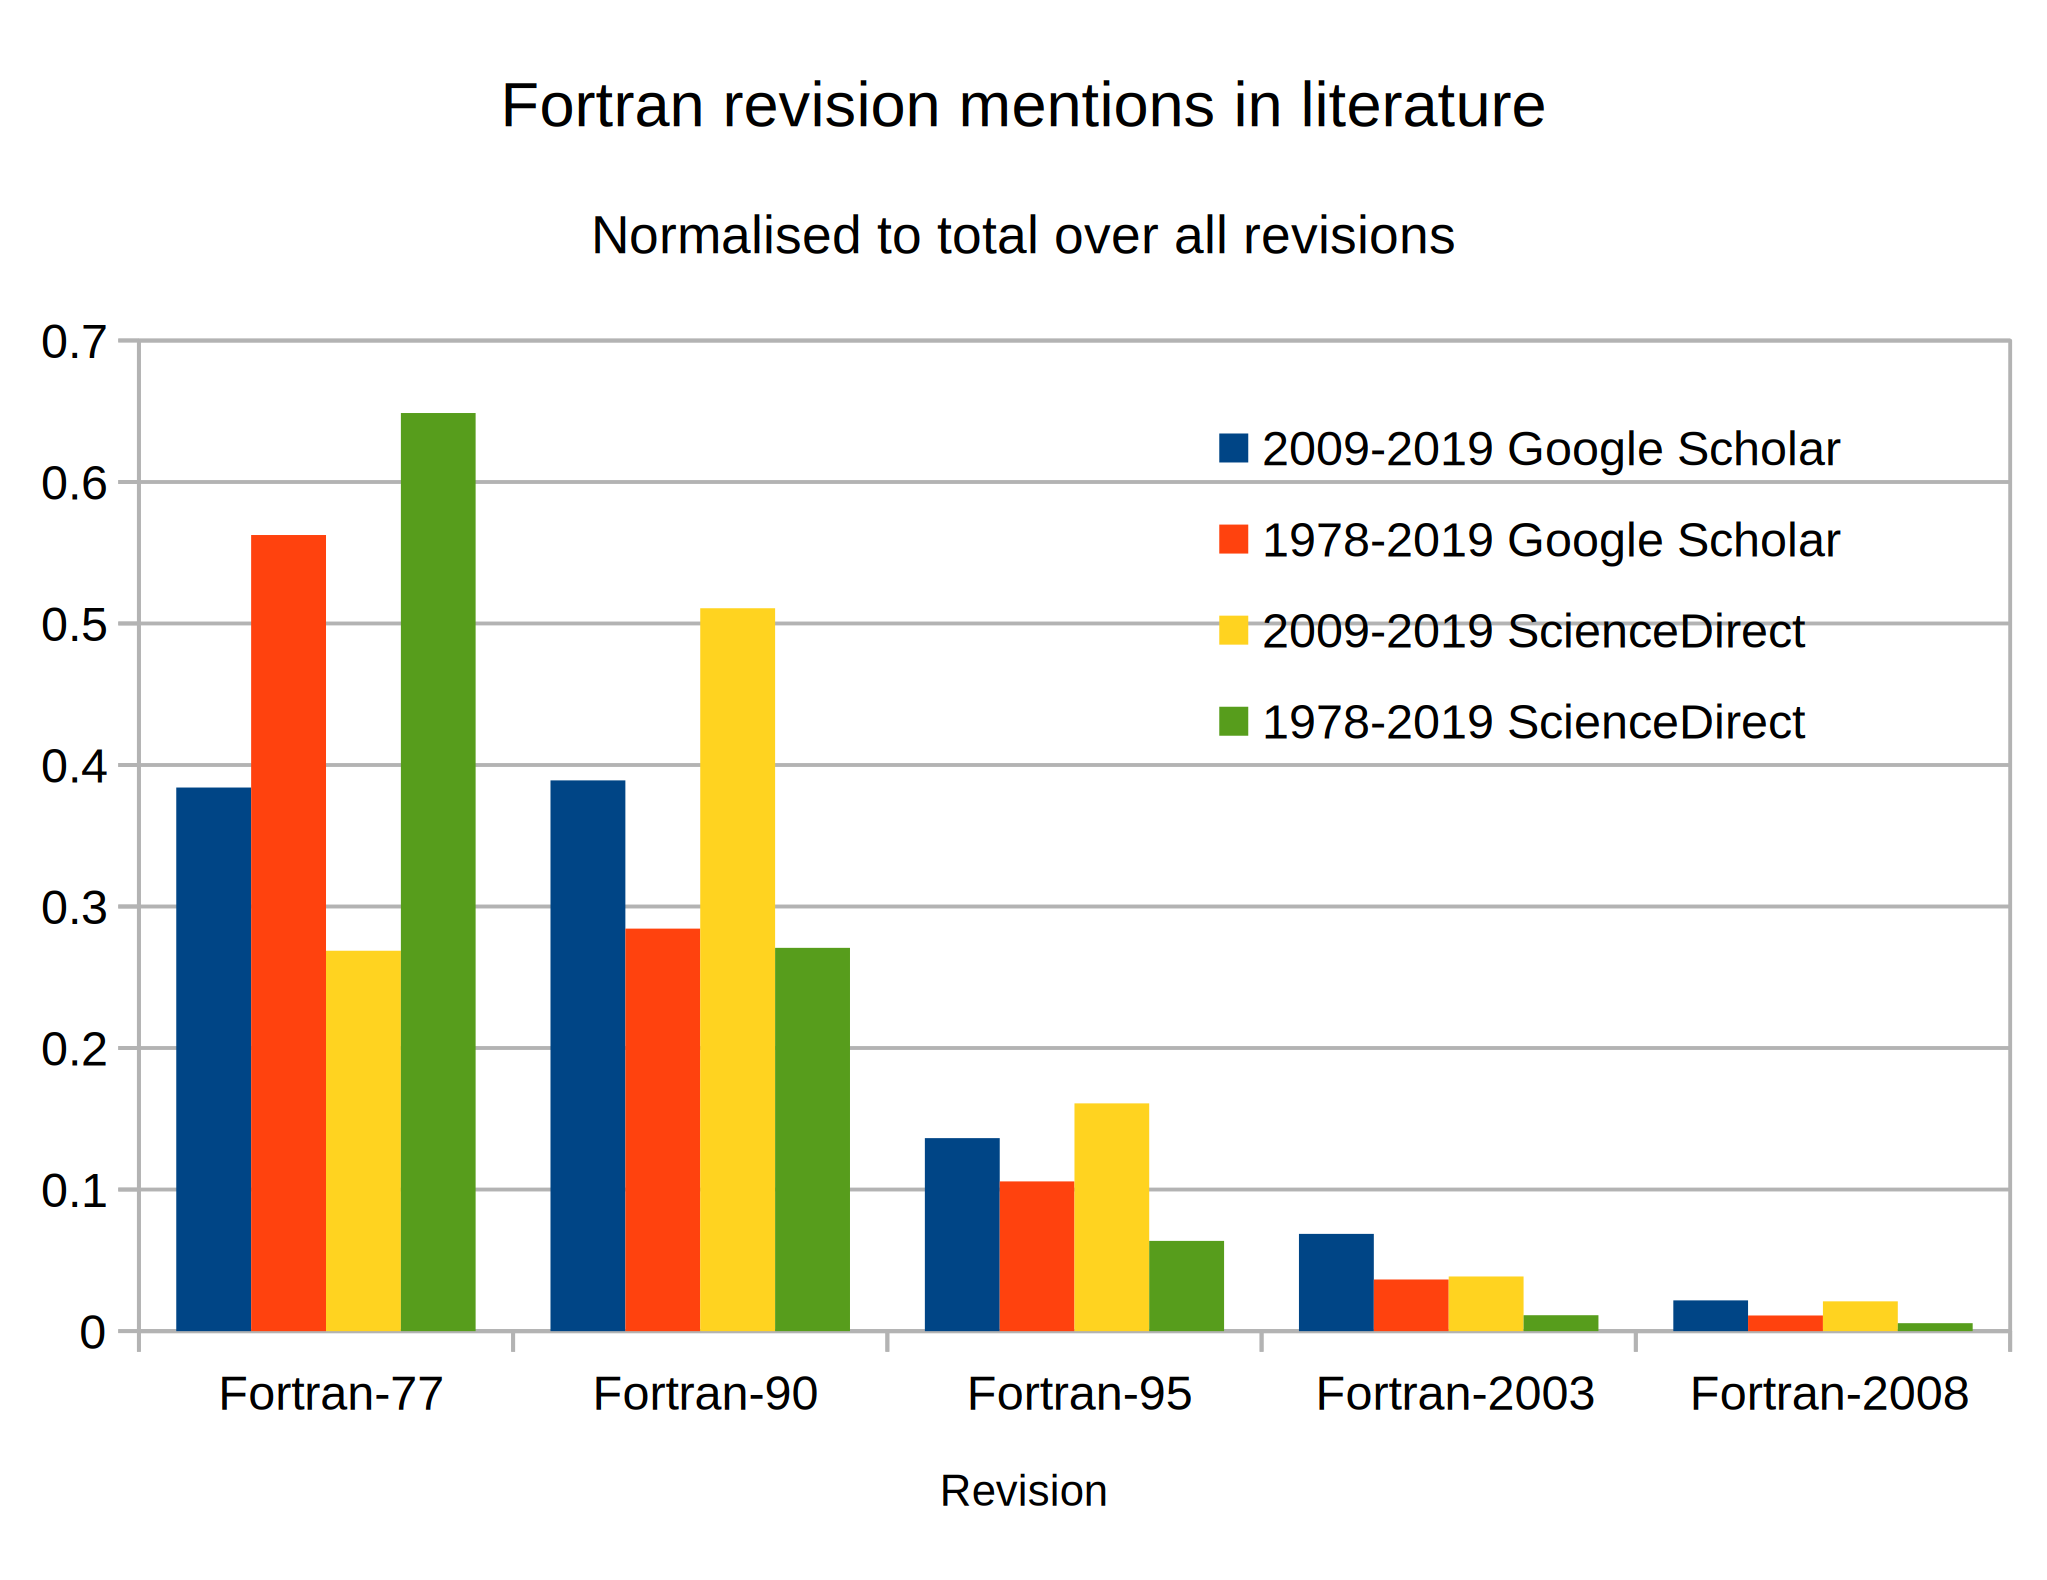
\includegraphics[width=0.71\textwidth]{fortran-versions-popularity-2019}\caption{Literature mentions of different revisions of Fortran using Google
Scholar and ScienceDirect\label{fig:Literature-mentions-of}}
\end{figure}

Based on the above evidence (confirmed by our own experience of collaboration
with scientists), the current state of affairs is that for many scientists,
FORTRAN 77 is still effectively the language of choice for writing
models. Even if the code adopts Fortran 90 syntax, in practice very
few of the semantic extensions are used, so that from a semantic perspective
the code is FORTRAN 77. There is also a vast amount of legacy code
in FORTRAN 77. Because the FORTRAN 77 language was designed with assumptions
and requirements very different from today, code written in it has
inherent issues with readability, scalability, maintainability and
parallelization. A comprehensive discussion of the issues can be found
in \cite{tinetti2012fortran}. As a result, many efforts have been
aimed at refactoring legacy code, either interactive or automatic,
and to address one or several of these issues. Our work is part of
that effort, and we are specifically interested in automatically refactoring
Fortran for offloading to accelerators such as GPUs and FPGAs.

\subsection{Acceleration by offloading matters}

Hardware accelerators have proven extremely effective in accelerating
scientific code. Of the \href{https://www.top500.org/lists/green500/2019/11/}{Green Top 10},
eight systems use accelerators. However, in practice the accelerators
have their own memory, and the most common compute model is still
to offload part of the calculation to the accelerator and copy the
results back to the host memory. Even if the accelerator is cache-coherent
with the host memory, having the code to be run on the accelerator
in a separate memory space is still advantageous as it results in
reduced coherency traffic.

\subsection{The need for pure functions}

Because of the separation of memory spaces and the absence of an operating
system on the accelerator, the code units offloaded to the accelerator
must be self-contained: 
\begin{itemize}
\item no shared memory space (\textsf{COMMON} blocks)
\item no system calls in general and no I/O operations in particular
\item no library calls except intrinsic ones 
\end{itemize}
A routine which meets these requirement is equivalent to a \emph{pure
function}: for a given set of input values, it always produces the
same outputs values, and it only influences the rest of the world
through these output values. Therefore, any other mechanism to share
data (specifically \textsf{COMMON} blocks) is not allowed.

A kernel offloaded to an accelerator is in general expected to behave
as a pure function: the inputs are the data copied to the accelerator's
memory and the outputs the data copied from the accelerator's memory.
Therefore, a key requirement for offloading code units to accelerators
is that they are pure functions. Note that this implies ``no I/O
system calls'' because these would cause the function to be impure.
The restriction on library calls is a practical one because they can't
be incorporated into the binary for the accelerator. From a ``pure
function'' perspective, calls to library functions are acceptable
if the library functions themselves are pure. 

\subsection{The case for type safety}

\subsubsection{What is type safety}

In his paper, ``A Theory of Type Polymorphism in Programming'' \cite{milner1978theory},
Robin Milner expressed the notion of type safety as \textquotedblleft Well
typed programs cannot go wrong.\textquotedblright{} By ``going wrong''
we mean in general not computing the expected result. There are several
components contributing to this behaviour: one is the language's type
system, the other is the type checker, and finally there is the actual
program code. 

In a type-safe language, the language\textquoteright s type system
ensures programs cannot perform operations that are not compatible
with the types of the operands involved, i.e. there are no type errors
in a well-typed program written in a type-safe language. By type error
we mean an error arising from the fact that a variable (or constant
or function) with a given type is treated as if it has a different
type. 

A type checker is called \emph{sound }if it only accepts correctly
typed programs. However, the fact that a sound type checker accepts
a correctly typed program does not mean the program is correct. 

\subsubsection{Type safety in Fortran}

In the context of Fortran, the type system as specified in ``ANSI
X3.9-1978 -- American National Standard Programming Language FORTRAN''
\cite{ansi1978standard}, hereafter called the ``f77 specification'',
is not type-safe. It is possible to write programs which the type
checker accepts but are nonetheless incorrect from the perspective
of the type system. The key culprit for this is the loss of type information
which occurs when data is handled via \textsf{COMMON} blocks or \textsf{EQUIVALENCE}
statements. 


\section{Related work}

\subsection{Formalisation of Fortran}

There has been surprisingly little research into Fortran's type system.
There is some work on formalisation of data abstraction, specifically
encapsulation to create abstract arrays in FORTRAN 77 \cite{54403}
and on the formal specification of abstract data types implemented
through derived types in Fortran 90 \cite{SCOTT1994201,MALEY1996167}.
There is also some work on the formalisation of Fortran 95 semantics
using VDM \cite{reid1999prescriptive} but there is no publication
on the final outcome. Specifically with regards to the type system,
the only work that we are aware of is on the extension of Fortran
90 types with an attribute reflecting the unit of measurement \cite{contrastin2016units}.
According to our survey, a formalisation of the FORTRAN 77 type system
or an analysis of its type safety has not been reported before.

\subsection{Source-to-source compilation and refactoring}

There are a number of source-to-source compilers and refactoring tools
for Fortran available. However, very few of them actually support
FORTRAN 77. The most well known are the ROSE framework\footnote{\url{http://www.rosecompiler.org/index.html}}
from LLNL \cite{liao2010rose}, which relies on the Open Fortran Parser
(OFP\footnote{\url{http://fortran-parser.sourceforge.net/}}). This
parser claims to support the Fortran 2008 standard. Furthermore, there
is the language-fortran\footnote{\url{https://hackage.haskell.org/package/language-fortran}}
parser which claims to support FORTRAN 77 to Fortran 2003. A  refactoring
framework which claims to support FORTRAN 77 is CamFort \cite{Orchard:2013:UFS:2541348.2541356},
according to its documentation it supports Fortran 66, 77, and 90
with various legacy extensions. That is also the case for the Eclipse-based
interactive refactoring tool Photran \cite{overbey2005refactorings},
which supports FORTRAN 77 - 2008. These tools are very useful, indeed
both CamFort and Photran provide powerful refactorings. As we shall
discuss in more detail below, for effective refactoring of common
blocks, and determination of data movement direction, whole-source
code (inter-procedural) analysis and refactoring is essential. A long-running
project which does support inter-procedural analysis is PIPS\footnote{\url{http://pips4u.org/}},
started in the 1990's. The PIPS tool does support FORTRAN 77 but does
not supported the refactorings we propose. For completeness we mention
the commercial solutions plusFort \footnote{\url{http://www.polyhedron.com/pf-plusfort0html}}
and VAST/77to90 \footnote{\url{http://www.crescentbaysoftware.com/compilertech.html}}
which both can refactor common blocks into modules but not into procedure
arguments. In conclusion, there are many projects that provide refactoring
program transformations. However, none of them focus on the type safety
of the resulting programs. 

\section{Contribution}

We present in this paper a formal analysis of the type safety of normalised
FORTRAN 77 programs (Section \ref{sec:Formal-analysis-of}) and a
series of algorithms for program transformation into normalised form
(Section \ref{sec:Program-transformations-for}). We also present
additional type checks for \textsf{COMMON} blocks and \textsf{EQUIVALENCE}
asociations (Section \ref{sec:Typechecking-COMMON-block}), as a precondition
to the program transformation.

These algorithms are implemented in our source-to-source compiler\footnote{\url{https://github.com/wimvanderbauwhede/RefactorF4Acc}}
which can automatically rewrite FORTRAN 77 programs into Fortran 90
so as to remove all \textsf{COMMON} and \textsf{EQUIVALENCE} statements,
provide full referential transparency and ensure that all functions
marked for offloading to accelerators are pure. 

We further show that (with a small number of additional restrictions),
the resulting code is type safe when type checked against the type
system which we present and well typed programs adhering to these
restrictions will not go wrong if they are accepted by the type checker.
What this means is that, if an original FORTRAN 77 program is accepted
by the type checker of our source-to-source compiler, then the Fortran
90 program which it generates can be type checked with an ordinary
Fortran compiler with all type-based warnings turned into errors,
and the code will type check cleanly. 


\section{Formal analysis of the type safety of normalised Fortran programs\label{sec:Formal-analysis-of}}

In this work, a \emph{normalised} FORTRAN 77 program is a program
that consists of pure functions (see Section \ref{subsec:The-definition-of}
for a formal definition) and where all variables, parameters and functions
are explicitly typed. We discuss in Section \ref{sec:Program-transformations-for}
how to achieve fully explicitly typing and under which conditions
a procedure can be made pure.

\subsection{Type systems concepts and notation\label{subsec:Type-systems-concepts}}

A \emph{type} is a formal mechanism to provide information about the
expected form of the result of a computation. More precisely, if \emph{e}
is an expression, a \emph{typing }of for e.g. $e:\mathrm{integer}$
is an assertion that when \emph{e} is evaluated, its value will be
an integer. Such an assertion is called a typing judgment. For such
a typing judgement to be meaningful, $e$ must be well typed. For
any expression this means that it must be internally consistent as
well as consistent with its context, i.e. if the expression $e$ contains
free variables, they must be declared with the right type in the context
of the code unit. We will use the term \emph{type statement} (as used
in the f77 specification) or \emph{type declaration} (more common
in type theory) for the statements that declare the type of a constant,
variable or function.

We use set theory to construct the sets of valid types for FORTRAN
77, and the standard notation for typing rules as used for example
in \cite{pierce2002types}, which can be summarised as: 
\begin{itemize}
\item The assertion ``the expression \emph{e} has type $\tau$'' is written
as $e:\tau$
\item If an assertion must hold for a certain context, i.e. a set of expressions
with declared types such as a code unit, the context is conventionally
denoted as $\Gamma$ and the operator $\vdash$ (called ``turnstyle''
in type theory) is used to write an assertion of the form ``assuming
a context $\Gamma$ then the expression \emph{e} has type $\tau$''
is written as $\Gamma\vdash e:\tau$ .
\item The double arrow ($\Rightarrow$) is used to put additional constraints
on a type and is read as ``these constraints must apply to the type
for the type judgement to hold''
\item The type of a function of a single argument is written as $f:\tau_{in}\rightarrow\tau_{out}$
and the function itself is written without parentheses, so $y=f\,x$
rather than $y=f(x)$.
\item We will write the type declaration for a tuple (ordered set) of \emph{m}
expressions as $(e_{1},...,e_{m}):(\tau_{1},...,\tau_{m})$ or for
brevity as $\mathbf{e_{m}}:\mathbf{T_{m}}$.
\end{itemize}
We deviate slightly from the terminology used in the f77 specification
in favour of the more common terminology: we will refer to the symbolic
name of a datum as a variable rather than a variable name, and we
will refer to what the f77 specification calls a variable as a scalar.
Thus a variable can be a scalar or an array. 

\subsection{The definition of a pure function\label{subsec:The-definition-of}}

If a function is pure, then it must return a least one datum as a
result, because otherwise it means it did not compute anything and
can be removed as dead code. Furthermore, a pure function without
input arguments is effectively a constant, so we can also assume that
the there is at least a single input variable. Therefore, we can without
loss of generality assume that a function takes as a single argument
a tuple of expressions, and returns a tuple of expressions. 

Let $\Gamma$ be the context of a given program, i.e. the set of all
variables with their type that are declared in a code unit:

\[
\Gamma=\{...,x_{i}:\tau_{i},...\}
\]

Consider a function 

\begin{eqnarray*}
f:(\tau_{in,1},...,\tau_{in,k}) & \rightarrow & (\tau_{out,1},...,\tau_{out,m})\\
(x_{out,1},...,x_{out,m}) & = & f\,(x_{in,1},...,x_{in,k})
\end{eqnarray*}

or shorter

\begin{eqnarray*}
f:\mathbf{T_{in,k}} & \rightarrow & \mathbf{T_{out,m}}\\
\mathbf{x_{out,k}} & = & f\,\mathbf{x_{in,m}}
\end{eqnarray*}

This function is \emph{pure} iff

\[
\forall\,\Gamma,\forall\mathbf{x_{in,k}}\in\Gamma,\exists!\,\mathbf{x_{out,m}}\in\Gamma:\mathbf{x_{out,m}}=f\mathbf{\,x_{in,k}}
\]

In words, for any given context $\Gamma$ where $\mathbf{x_{in,k}}$
and $\mathbf{x_{out,m}}$ are declared, then if $\mathbf{x_{in,k}}$
is a given set of argument values of the correct type, the function
will always return the same values $\mathbf{x_{out,m}}$ regardless
of the rest of the content of $\Gamma$. Note that the fact that $\Gamma$is
the same for the inputs$\mathbf{x_{in,k}}$ and the results of the
function call $\mathbf{x_{out,m}}$ implies that the function does
not modify $\Gamma$. We will see in Section \ref{sec:Program-transformations-for}
and following how any Fortran procedure can be transformed into a
pure function.


\subsection{Specification of FORTRAN 77 data types\label{subsec:Specification-of-FORTRAN}}

According to �4.1 \emph{Data Types} of the f77 specification, 

\begin{quote}

The six types of data are:
\begin{enumerate}
\item Integer
\item Real
\item Double precision
\item Complex
\item Logical
\item Character
\end{enumerate}
\end{quote}

The f77 specification discusses each of these types in terms of their
\emph{storage units}. According to �2.13 \emph{Storage}: 
\begin{quote}
A storage unit is either a numeric storage unit or a character storage
unit. An integer, real, or logical datum has one numeric storage unit
in a storage sequence. A double precision or complex datum has two
numeric storage units in a storage sequence. A character datum has
one character storage unit in a storage sequence for each character
in the datum. This standard does not specify a relationship between
a numeric storage unit and a character storage unit. If a datum requires
more than one storage unit in a storage sequence, those storage units
are consecutive.
\end{quote}
Thus
\begin{itemize}
\item An integer or real has one storage unit
\item A \emph{double precision} datum has two consecutive numeric storage
units in a storage sequence (�4.5 \emph{Double Precision Type}).
\item A \emph{complex} datum is a processor approximation to the value of
a complex number. The representation of a complex datum is in the
form of an ordered pair of real data. The first of the pair represents
the real part of the complex datum and the second represents the imaginary
part. Each part has the same degree of approximation as for a real
datum. A complex datum has two consecutive numeric storage units in
a storage sequence; the first storage unit is the real part and the
second storage unit is the imaginary part (�4.6 \emph{Complex Type}).
\end{itemize}
As quoted above, the f77 specification does not specify the size of
a storage unit. However, the consensus amongst the major Fortran compilers\footnote{GNU, PGI/Nvidia, Intel, SunSoft/Oracle, Lahey/Fujitsu}
is as follows:

\begin{table}[h]
\begin{centering}
\begin{tabular}{|c|c|c|}
\hline 
Type & Size in bytes (Kind) & \#Storage Units (numeric)\tabularnewline
\hline 
\hline 
\texttt{integer} & 4 & 1\tabularnewline
\hline 
\texttt{real} & 4 & 1\tabularnewline
\hline 
\texttt{double precision} & 8 & 2\tabularnewline
\hline 
\texttt{complex} & 8 & 2\tabularnewline
\hline 
\texttt{logical} & 4 & 1\tabularnewline
\hline 
 & Size in bytes & \#Storage Units (character)\tabularnewline
\hline 
\texttt{character} & 1 & 1\tabularnewline
\hline 
\end{tabular}
\par\end{centering}
\caption{Relationship between storage unit, kind and bytes for FORTRAN 77 types.\label{tab:Relationship-between-storage}}
\end{table}

Various extensions exists such as \texttt{byte}, \texttt{double complex}
etc. Technically, the use of \emph{kinds} in type declarations (e.g.
\texttt{integer{*}8}) is not part of the f77 specification. It is
however widely used and supported by all current Fortran compilers,
specifically the open source GNU Fortran compiler g77. In this paper
we effectively consider FORTRAN 77 to be defined by the f77 specification
combined with the g77 extensions\footnote{\href{https://gcc.gnu.org/onlinedocs/gcc-3.4.6/g77/Language.html}{https://gcc.gnu.org/onlinedocs/gcc-3.4.6/g77/Language.html}}. 

We will treat the \emph{kind} as the number of bytes of storage as
in Table \ref{tab:Relationship-between-storage} and define the scalar
types as \emph{(Typename, Kind)} tuples. Moreover, we define a character
storage unit as 1 byte. This allows us the simplify the types to integer,
real, complex and logical, because we can define a double precision
as (real,8) and a character as (integer,1). For the rest of the discussion
we will treat the character type as an integer with a kind of 1 and
a character string as an array of characters. We will not discuss
any special cases for characters because it would needlessly complicate
the discussion without adding anything material in terms of the type
system.

\subsection{Formalising the FORTRAN 77 type system }

With the conventions from Section \ref{subsec:Specification-of-FORTRAN}
and the above assumptions, we can describe Fortran's type system using
sets of entities as show in Definition \ref{alg:The-FORTRAN-77}.
\begin{definition}
The FORTRAN 77 type system for scalars and arrays\label{alg:The-FORTRAN-77}

Type = $\left\{ Integer,Real,Complex,Logical\right\} $ 

NumType = $\left\{ Integer,Real,Complex\right\} $ 

Kind = $\left\{ 2^{n}|\;n\in[0,5]\right\} $

Scalar = $\left\{ Type\times Kind\right\} $, an element is denoted
as \emph{Scalar t k} or \emph{t{*}k}

Num = $\left\{ NumType\times Kind\right\} $, an element is denoted
as \emph{Num a}

Bool= $\left\{ Logical\times Kind\right\} $, an element is denoted
as \emph{Bool}

Dim =$\left\{ ((b_{i},e_{i}),...,(b_{i},e_{i}),...,(b_{k},e_{k})),\forall k,i\in\,[1,7],b_{i},e_{i}\in\mathbb{Z},b_{i}\le e_{i}\right\} $,
so Dim is a set of ordered sets of tuples, we denote an element as
\emph{Dim d}

Array = $\left\{ Scalar\times Dim\right\} $, and we denote an element
of this set as \emph{Array (Scalar t k) (Dim d)}

FortranType = $Scalar\cap Array$ 

Tuple = ($\tau\times...\times\tau_{i}\times...\times\tau_{k}),\,\forall\,i\,\in[1,k]\,|\,\tau_{i}\in\mathit{FortranType}$
and we'll write \emph{Tuple t}, where $t=(\tau_{1},...,\tau_{k})$
\end{definition}
With the organisation in Definition \ref{alg:The-FORTRAN-77}, the
general form of a type $\tau$ in Fortran 77 is given as
\begin{definition}
\label{def:General-form-a}General form a type $\tau$ in Fortran
77

\begin{eqnarray}
\tau & ::=\\
 & FortranType & \textrm{primitive\,type}\nonumber \\
| & Tuple & \textrm{tuple\,type}\nonumber \\
| & \tau\rightarrow\tau & \textrm{function\,type}\nonumber \\
| & void & \textrm{non-type}\nonumber \\
| & a & \textrm{type\,variable}\nonumber 
\end{eqnarray}
\end{definition}
The type variables arise a result of the polymorphism of the arithmetic
and relational operators, as well as of some intrinsic functions.
The \emph{void} type is used in the typing rules for subroutine calls
and assignments, as these are statements that do not have a type.

To investigate the type safety of this type system, we need to consider
the typing rules for
\begin{itemize}
\item Constants
\item Scalar and array declarations and accesses
\item Function and subroutine declarations and applications
\item Assignments
\item Expressions
\end{itemize}
Furthermore, we need to consider specifically how Fortran handles
subtypes, which arise in the context of what the f77 specification
calls \emph{type conversion}, also commonly known as type coercion.

\subsubsection{Constants}

The forms of numeric constants are described in words in �4 \emph{Data
Types and Constants} of the f77 specification. Using Extended Backus-Naur
Form (EBNF, \footnote{\href{https://www.w3.org/TR/2008/REC-xml-20081126/\#sec-notation}{https://www.w3.org/TR/2008/REC-xml-20081126/\#sec-notation}}),
we can describe them formally as show in Definition \ref{alg:EBNF-for-numeric}.
\begin{definition}
EBNF for numeric constants\label{alg:EBNF-for-numeric}

integer-constant ::= {[}sign{]} \{digit\}+ 

sign ::= + | -

digit ::= 0 | 1 | 2 | 3 | 4 | 5 | 6 | 7 | 8 | 9

real-constant ::= {[}sign{]} \{digit\}{*} decimal-point \{digit\}{*}
{[}real-exponent{]}

| {[}sign{]} \{digit\}+ {[}decimal-point \{digit\}{*}{]} real-exponent

decimal-point ::= .

real-exponent ::= E {[}sign{]} \{digit\}+

double-constant ::= {[}sign{]} \{digit\}{*} decimal-point \{digit\}{*}
{[}double-exponent{]}

| {[}sign{]} \{digit\}+ {[}decimal-point \{digit\}{*}{]} double-exponent

double-exponent ::= D {[}sign{]} \{digit\}+

complex-constant ::== ( real-constant , real-constant )

logical-constant ::== .TRUE. | .FALSE.
\end{definition}
We define the set of constants of for each type, for example for integers:

\[
IntegerConstants=\left\{ n\,|\,n\,\textrm{is an integer-constant}\right\} 
\]

and thus we can write the typing rule

\[
\frac{\,}{n\,:\,Integer}.\,\forall\,n\in\mathit{IntegerConstants}
\]

\begin{description}
\item [{and}] similar for the other types.
\end{description}

\subsubsection{Scalars}

The typing rule for a scalar \emph{s} is simply that any access of
a scalar variable, this variable must have the same type, which must
be the type from its declaration in the current context (code unit)
$\Gamma$ and belong to the set \emph{Scalar}. We write this as

\[
\frac{\,}{\Gamma\vdash s:\tau_{s}=Scalar\,t\,k}
\]

What this means is that, given the context $\Gamma$ which contains
all types of all variables valid in a given expression, the type judgement
is valid. In a Fortran expression this means that all variables with
a type statement in a code unit will be of the type determined by
that statement. 

\subsubsection{Arrays}

The typing rule for an array declaration is that in addition to being
of a valid Scalar type 
\begin{itemize}
\item it must have a non-empty Dim set $Dim\,d$ :

\begin{align*}
\frac{\,}{\Gamma\vdash a:\tau_{a}=Array\,(Scalar\,t_{a}\,k_{a})\ (Dim\,d)}
\end{align*}

where $d=((b_{1},e_{1}),...,(b_{i},e_{i}),...,(b_{k},e_{k}))$ as
defined in Definition \ref{def:General-form-a}.
\item and for any array access $a(j_{1},...,j_{k}),j_{i}\in[b_{i},e_{i}]$ 
\begin{itemize}
\item the number indices must $k=\#d$, 
\item the type must be the scalar type:
\end{itemize}
\begin{align*}
\frac{\Gamma\vdash a:\tau_{a}\;\;\;\Gamma\vdash j_{i}:Integer,\forall\,i\in[1,k]}{\Gamma\vdash a(j_{1},...,j_{i},...,j_{k}):\tau_{s}=Scalar\,t_{a}\,k_{a}}
\end{align*}

\end{itemize}
Note that the additional condition of validity of the range of the
array indices $a(j_{1},...,j_{i},...,j_{k}),\,\forall\,i\in[1,k]|j_{i}\in[b_{i},e_{i}]$
is not a type checking condition but an run-time range checking condition,
so it is not part of the typing rules.

\paragraph{Array slicing}

Fortran 90 allows array slicing using the notation $(b_{s}:e_{s}:s_{s})$,
and it is quite common in FORTRAN 77 style code. For example:
\begin{example}
Array slicing\label{exa:Array-Slicing}

\texttt{\small{}integer a, s}{\small\par}

\texttt{\small{}dimension a(5,7), s(3)}{\small\par}

\texttt{\small{}s = a(2,1:5:2)}{\small\par}
\end{example}
The array s will be populated with the values from \emph{a(2,1)},
\emph{a(2,3)} and \emph{a(2,5)}. From a type checking perspective,
we need to check if the slice has the correct type, in this case the
same type as the array to which it is assigned.

For a given tuple $(b_{i},e_{i})$ from \emph{d}, a slice is valid
(i.e. within bounds) if $b_{s}\geq b_{i},e_{s}\leq e_{i},s_{s}\leq e_{i}-b_{i}$.
We will call the set of indices in the slice a \emph{DimSlice} and
it is given by

\[
\mathit{DimSlice}=\left\{ idx|idx\in[b,e]\land(idx-b)\,mod\,%s=0
\right\} 
\]

and we'll denote this as \emph{DimSlice b e s}. 

The type of a sliced array is determined from the \emph{DimSlice}
as follows: 
\begin{itemize}
\item let the array \emph{a} have \emph{Dim d}, $d=(p_{1},...,p_{i},...,p_{k})$
and we slice the tuple $p_{i}$ with a valid slice $s_{i}=\mathit{DimSlice}\,b_{s}e_{s}s_{s}$.
\item Then this results in a new $p'_{i}=(1,\#s_{i})$ 
\item and therefore a new \emph{Dim d}', $d'=(p_{1},...,p'_{i},...,p_{k})$ 
\item and thus a new array type

\[
\tau'_{a}=Array\,\tau_{s}\ (Dim\,d')
\]

\end{itemize}
To be type safe, the size of the \emph{DimSlice} must be known at
type check time. This implies that the components \emph{b, e, s} of
the slice must be constant. If so, we can determine the size of the
slice and thus check that the new type is correct given the context.
In practice, our compiler performs aggressive linear constant folding,
which means that an linear expression with constants as leaf nodes
will be reduced to a constant. If the size of the \emph{DimSlice}
is only known at run time, our compiler allows to insert run-time
checks as explained in Appendix A1.

\paragraph{Arrays as indices}

Fortran also allows arrays to be indexed by other arrays, for example
\begin{example}
Arrays as indices

\texttt{\small{}integer a(5,5), b(3), k(3)}{\small\par}

\texttt{\small{}k = (/ 1, 5, 2 /)}{\small\par}

\texttt{\small{}b = a(2, k)}{\small\par}
\end{example}
The array \emph{b} will contain the values from \emph{a(2,1)}, \emph{a(2,5)}
and \emph{a(2,2)} in that order.

The array to be used for indexing must be an array of rank 1 that
contains the indices of the locations to be accessed, just like a
\emph{DimSlice}. Thus the requirement for type safety is the same
(the size of the array), and the criterion for the array to be valid
for indexing is that all elements must be in the valid index range
for the given array index. If the index range is only known at run
time, our compiler allows to insert run-time checks as explained in
Appendix A2.

\paragraph{Bounds checking}

Fortran checks constant array bounds at type check time and our compiler
performs a more aggressive constant folding so that any index reducible
to a constant with linear arithmetic will be considered constant.
However, in general array indices are not known at type check time
and therefore even in a well typed program, it is still possible to
have out-of-bound errors. Fundamentally, index checking is not type
checking because it concerns the actual values, and has to be performed
at run time. All modern Fortran compilers provide this option, e.g.
\texttt{-fcheck=bounds} in the GNU gfortran.

\subsubsection{Subroutines and Functions}

As explained below (Section \ref{subsec:The-definition-of}), every
Fortran subroutine or external function can be transformed into a
pure function. Intrinsic functions are pure by definition. From a
type checking perspective, the difference between a Fortran function
(external or intrinsic) and subroutine is that a function call can
occur in an expression, and therefore has a return type, and a subroutine
call is a statement and so has no return type. As explained before,
we consider both subroutines and functions to be pure in the sense
that any interaction with the code is via the arguments and return
value.

The subroutine declaration typing rule is that every dummy argument
must be of a valid \emph{FortranType}. A subroutine does not return
a type, we denote this by using \emph{void}. Using the tuple type
notation from Section \ref{subsec:Type-systems-concepts}, we write
this as:

\[
\frac{\,}{FortranType\,\mathbf{T_{k}}\Rightarrow sf:\mathbf{T_{k}}\rightarrow void}
\]

The subroutine application (\texttt{call}) typing rule is that every
call argument and every dummy argument must have the same type. Because
a subroutine call is a statement, it does not return a type:

\[
\frac{FortranType\,\mathbf{T_{k}}\Rightarrow sf:\mathbf{T_{k}}\rightarrow void\;\;\;\Gamma\vdash\mathbf{e_{k}}:\mathbf{T_{k}}}{\Gamma\vdash\mathtt{call}\,sf\,e_{k}:void}
\]

The external function declaration typing rule is that every dummy
argument must be of a valid \emph{FortranType}. An external function
must have a return a type. Using the tuple type notation from Section
\ref{subsec:Type-systems-concepts}, we write this as:

\[
\frac{\,}{FortranType\,\mathbf{T_{k}},\tau_{f}\Rightarrow f:\mathbf{T_{k}}\rightarrow\tau_{f}}
\]

The function application typing rule is also that every call argument
and every dummy argument must have the same type. In that case, the
function application is of the type of the return type:

\[
\frac{FortranType\,\mathbf{T_{k},\tau_{f}}\Rightarrow f:\mathbf{T_{k}}\rightarrow\tau_{f}\;\;\;\Gamma\vdash\mathbf{e_{k}}:\mathbf{T_{k}}}{\Gamma\vdash f\,\mathbf{e_{k}}:\tau_{f}}
\]


\paragraph{Higher-order functions}

In the above we have glossed over one important detail: subroutines
and external functions can take the names of other subroutines or
external functions as arguments. The case of an external functions
is covered by the above typing rules because the function passed as
argument has as type the return type, and as such is indistinguishable
from a variable. A subroutine passed as an argument however does not
have a type, so we have to add \emph{void} to the set of types that
can are valid for arguments of a subroutine or function. 

In the case of a subroutine call:

\[
\frac{FortranType\cap\{void\}\,\mathbf{T_{k}}\Rightarrow sf:\mathbf{T_{k}}\rightarrow void\;\;\;\Gamma\vdash\mathbf{e_{k}}:\mathbf{T_{k}}}{\Gamma\vdash\mathtt{call}\,sf\,e_{k}:void}
\]

\[
\frac{FortranType\,\mathbf{T_{k}}\Rightarrow sf:void\rightarrow void\;\;\;\Gamma\vdash\mathbf{e}:\mathbf{T_{k}}\rightarrow void}{\Gamma\vdash\mathtt{call}\,sf\,e:void}
\]

and similar for a function call, purely for the sake of type checking
of the call. 

The f77 specification �8.7 \emph{EXTERNAL Statement} requires that
any external function or subroutine used as an argument is declared
using the \textsf{EXTERNAL} statement. Omitting this declaration results
in a type error. 

Strictly speaking this means that \emph{External} is a type attribute
for functions or subroutines, in other words the type of a function
in Definition \ref{def:General-form-a} must be extended with this
attribute:

\[
f:(\mathit{External},\tau\rightarrow\tau)
\]

with

\[
\mathit{External}=\mathit{True\,}|\,\mathit{False}
\]

However, for the purpose of this paper we will maintain the unextended
type and instead group the \textsf{EXTERNAL} functions in a separate
context. The actual type checking of higher-order functions is not
possible at compile time. In Appendix A3, we present an algorithm
for run-time type checking via the construction of a sum type of the
higher-order functions in a compute unit.

\subsubsection{Assignments}

Because in Fortran the assignment is a statement, it does not return
a type. Therefore, the type check rule for an assignment ($\leftarrow$)
of a variable \emph{v} declared in the context $\Gamma$ to an expression
\emph{e} which may contain any variable $v_{i}$ declared in the context
$\Gamma$, is as follows:

\[
\frac{\Gamma\vdash v:\tau\;\;\;\Gamma(v_{i})\vdash e(v_{i}):\tau}{\Gamma\vdash v\leftarrow e:\,void}
\]

According to the f77 specification, only assignments to variables
and array elements are valid, but the extension to arrays as in Fortran
90 is very common. The above typing rule does not limit the type check
to scalars, so array assignments will type check if the types match.

\subsubsection{Expressions}

Expressions can consist of constants, variables, operators and calls
to intrinsic or external functions. 

\paragraph{Polymorphic numeric operators}

Numeric operators in Fortran are \emph{polymorphic}, i.e. they can
handle operands of any \emph{Num} type.
\begin{itemize}
\item The operators \texttt{+},\texttt{-},\texttt{{*}} have type:

\[
Num\,a\Rightarrow a\rightarrow a\rightarrow a
\]
Given that \emph{a} is a valid \emph{Num} type (see Definition \ref{alg:The-FORTRAN-77})
then the operator takes two arguments of type \emph{a} and returns
an argument of type \emph{a}. 
\begin{itemize}
\item The operator \texttt{{*}{*}} also has the type 
\[
Num\,a\Rightarrow a\rightarrow a\rightarrow a
\]
\end{itemize}
except when the exponent is an integer, in which case the type is: 

\[
\mathit{Kind}\,k,\,\mathit{Num}\,a\Rightarrow a\rightarrow\mathit{Integer}*k\rightarrow a
\]

\item The unary \texttt{-} operator is also polymorphic with type
\end{itemize}
\begin{center}
$Num\,a\Rightarrow a\rightarrow a$
\par\end{center}
\begin{itemize}
\item In Fortran 90, all the above operators also work on arrays, i.e. we
have
\begin{center}
$Num\,a,Dim\,d\Rightarrow Array\,a\,d\rightarrow Array\,a\,d\rightarrow Array\,a\,d$
\par\end{center}
\item Comparison operations .lt., .le.,.eq.,.ne.,.gt.,.ge. are all of type
\noindent \begin{center}
$Num\,a\Rightarrow a\rightarrow a\rightarrow Bool$
\par\end{center}
\end{itemize}

\paragraph{Polymorphic intrinsics }

Many intrinsic functions are also polymorphic. For the types of intrinsic
functions, we refer to Table 5 in the f77 specification. 
\begin{itemize}
\item Intrinsics are either of type
\begin{center}
$Num\,a\Rightarrow a\rightarrow a$ 
\par\end{center}

except for
\begin{center}
$\mathtt{imag}:\mathit{Kind}\,k\Rightarrow\mathit{Complex}*k\rightarrow\mathit{Real}*k$ 
\par\end{center}

\noindent or of type
\noindent \begin{center}
$\mathit{Num}\,a\Rightarrow a\rightarrow a\rightarrow a$
\par\end{center}

except for
\end{itemize}
\noindent \begin{center}
$\mathtt{dprod}:\mathit{Real}*4\rightarrow\mathit{Real}*4\rightarrow\mathit{Real}*8$ 
\par\end{center}
\begin{itemize}
\item The intrinsics \textsf{min} and \textsf{max} take a list of arguments
of a given type and undetermined length (denoted by $[...]$) 
\noindent \begin{center}
$\mathit{Num}\,a\Rightarrow[a]\rightarrow a$ 
\par\end{center}

except
\noindent \begin{center}
$\mathtt{amin0,amax0}:[\mathit{Integer}*4]\rightarrow\mathit{Real}*4$\\
$\mathtt{min1,max1}:[\mathit{Real}*4]\rightarrow\mathit{Integer}*4$
\par\end{center}
\end{itemize}

\paragraph{Expression type rule}

\noindent The expression forms a tree of applications of either operators
or intrinsic functions, with the leaves being constants or variables.
Type checking is performed via recursive descent, for example for
the \texttt{+} operator:

\[
\frac{Num\,a\;\;\;\Gamma\vdash e_{1}:a\;\;\;\Gamma\vdash e_{2}:a\;\;\;(+):a\rightarrow a\rightarrow a}{\Gamma\vdash e_{1}+e_{2}:\,a}
\]


\subsubsection{Type conversions for polymorphic operators }

The f77 specification defines specific intrinsic functions \texttt{int},
\texttt{real}, \texttt{dble} and \texttt{cmplx} for the purpose of
type conversion (Table 5), and the Fortran 90 specification extends
these to include the \emph{kind} (thereby making \texttt{dble} redundant).
Their signatures are respectively\footnote{The actual signature for \texttt{cmplx} is more complicated because
it can be used to construct a complex number from two reals, but for
the purpose of type conversion, the presented signature suffices.}:

\begin{align*}
\mathtt{int} & :Num\,a,Kind\,k\Rightarrow a\rightarrow k\rightarrow Integer*k\\
\mathtt{real} & :Num\,a,Kind\,k\Rightarrow a\rightarrow k\rightarrow Real*k\\
\mathtt{cmplx} & :Num\,a,Kind\,k\Rightarrow a\rightarrow k\rightarrow Complex*k
\end{align*}

As the name and the kind argument identify a Num type, for the typing
rules we use the generic notation\footnote{In Fortran 90, the type conversion functions can take an array operand:

$cast\langle\tau_{2}\rangle:Num\,\tau_{1},\tau_{2},Dim\,d\Rightarrow Array\,\tau_{1}\,d\rightarrow Array\,\tau_{2}\,d$}

\[
cast\langle\tau_{2}\rangle:Num\,\tau_{1},\tau_{2}\Rightarrow\tau_{1}\rightarrow\tau_{2}
\]

Fortran allows implicit type conversions (coercion) for operators
and assignments, according to some simple \emph{subtyping} rules. 

A type $\tau_{1}$is a subtype of a type $\tau_{2}$ if it is safe
to use a term of type $\tau_{1}$ in an context that expects a term
of type $\tau_{2}$. We denote this as $\tau_{1}<:\tau_{2}$ . 

The following (transitive) subtyping relations apply to numeric Fortran
types:

\begin{eqnarray*}
Integer*k & <: & Real*k,k\in Kind\\
Real*k & <: & Complex*k\\
t*k_{1} & <: & t*k_{2},k_{1},k_{2}\in Kind,t\in NumType
\end{eqnarray*}

Therefore we can write the type conversion rules from Table 2 \emph{Type
and Interpretation of Result for $x_{1}+x_{2}$} of the f77 specification
formally as

\[
\frac{\begin{array}{ccc}
 & Num\,\tau_{1},\tau_{2}\\
 & \tau_{1}<:\tau_{2}\\
\Gamma\vdash e_{1}:\tau_{1} & \Gamma\vdash e_{2}:\tau_{2} & op:Num\,a\Rightarrow a\rightarrow a\rightarrow a
\end{array}}{\Gamma\vdash op\;cast\langle\tau_{2}\rangle\,e_{1}\;e_{2}:\tau_{2}}
\]

with \emph{op} = +,-,{*},/ or {*}{*} \footnote{unless the exponent of \texttt{{*}{*}} is an integer, in which case
there is no type conversion}. 

If the types of the arguments are such that $\tau_{2}<:\tau_{1}$
then the cast applies to the second argument.

As for the relational operators .lt., .le., .eq., .ne., .gt., .ge.,
according to the f77 specification �6.3.3 \emph{Interpretation of
Arithmetic Relational Expressions}:
\begin{quote}
If the two arithmetic expressions are of different types, the value
of the relational expression \texttt{e1 relop e2} is the value of
the expression \texttt{((e1) - (e2)) relop 0}
\end{quote}
Therefore the type conversion rules is very similar:

\[
\frac{\begin{array}{ccc}
 & Num\,\tau_{1},\tau_{2}\\
 & \tau_{1}<:\tau_{2}\\
\Gamma\vdash e_{1}:\tau_{1} & \Gamma\vdash e_{2}:\tau_{2} & relop:Num\,a\Rightarrow a\rightarrow a\rightarrow Bool
\end{array}}{\Gamma\vdash relop\;cast\langle\tau_{2}\rangle\,e_{1}\;e_{2}:Bool}
\]


\subsubsection{Type conversion of assignments}

For assignments, the f77 specification states that the assignment
is typed according the following rules:
\begin{quote}
Execution of an arithmetic assignment statement causes the evaluation
of the expression e by the rules in Section 6, conversion of e to
the type of v , and definition and assignment of v with the resulting
value, as established by the rules in Table 4.
\end{quote}
This means that, if the subtyping relationship holds, we have:

\[
\frac{\begin{array}{ccc}
 & Num\,\tau_{1},\tau_{2}\\
 & \tau_{2}<:\tau_{1}\\
\Gamma\vdash v:\tau_{1} & \Gamma(x_{i})\vdash e(x_{i}):\tau_{2}
\end{array}}{\Gamma\vdash v\leftarrow cast\langle\tau_{1}\rangle\,e:void}
\]

However, if the subtyping relationship does \emph{not} hold, we have:

\[
\frac{\begin{array}{ccc}
 & Num\,\tau_{1},\tau_{2}\\
 & \tau_{1}<:\tau_{2}\\
\Gamma\vdash v:\tau_{1} & \Gamma(x_{i})\vdash e(x_{i}):\tau_{2}
\end{array}}{\Gamma\vdash v\leftarrow cast\langle\tau_{1}\rangle\,e:void}
\]

In other words, \emph{e} is implicitly converted to the type of \emph{v}
even if the conversion is unsafe. Strictly speaking, this is a type
error, and if we type check e.g. Example \ref{exa:Unsafe-coercion}
using the GNU fortran compiler with flags as shown in Example \ref{exa:Output-from-g77},
we do indeed get a type error. 
\begin{example}
Unsafe coercion\label{exa:Unsafe-coercion}

\texttt{\small{}program unsafeCoercion}{\small\par}

\texttt{\small{}~~integer i1,i2}{\small\par}

\texttt{\small{}~~real r1}{\small\par}

\texttt{\small{}~~r1 = 0.14159}{\small\par}

\texttt{\small{}~~i1=3}{\small\par}

\texttt{\small{}~~i2 = i1+r1}{\small\par}

\texttt{\small{}end}{\small\par}
\end{example}
~
\begin{example}
Output from g77 for program \texttt{unsafeCoercion\label{exa:Output-from-g77}}

\texttt{\footnotesize{}g77 -fsyntax-only -Werror=conversion test\_type\_coercion.f}{\footnotesize\par}

\texttt{\footnotesize{}test\_type\_coercion.f:6:11:}{\footnotesize\par}

\texttt{\footnotesize{}6 | i2 = i1+r1}{\footnotesize\par}

\texttt{\footnotesize{}| 1}{\footnotesize\par}

\texttt{\footnotesize{}Error: Possible change of value in conversion
from REAL(4) to INTEGER(4) at (1) {[}-Werror=conversion{]}}{\footnotesize\par}
\end{example}
However, this behaviour is so common that by default, Fortran compilers
only warn about unsafe conversions, and then only when warnings are
enabled. Our compiler warns by default and converts the implicit type
conversion to an explicit conversion as shown in Example \ref{exa:Explicit-conversion}.
Thus the resulting code is type safe, and we assume that the explicit
conversion is what the programmer wants.
\begin{example}
Explicit conversion\label{exa:Explicit-conversion}

\texttt{\small{}program unsafeCoercion}{\small\par}

\texttt{\small{}$\,$~~integer :: i1,i2}{\small\par}

\texttt{\small{}~~real :: r1}{\small\par}

\texttt{\small{}~~r1 = 0.14159}{\small\par}

\texttt{\small{}~~i1=3}{\small\par}

\texttt{\small{}~~i2 = int(i1+r1,4)}{\small\par}

\texttt{\small{}end program unsafeCoercion}{\small\par}
\end{example}

\subsection{Conclusions regarding the type safety of the Fortran type system}

Based on the above analysis, we conclude that FORTRAN 77 programs
that are explicitly typed and consist of pure functions are type safe,
except for three specific constructs: array slicing and array indexing
with values that are unknown at compile time, and higher-order functions.
Current compilers guarantee type safety if the slice indices or the
arrays used as index are constant, and also if the array used for
indexing is of the wrong rank. However, if the indices are non-constant
expressions, potentially unsafe programs pass without warning or error.
Our compiler will issue a type error, which can be relaxed to warning
or run-time type check, rather than ignoring the potential unsafe
behaviour. 

Calls to functions passed as arguments to other functions (i.e. higher-order
functions) are fundamentally unsafe because the type signature of
Fortran functions and subroutines does not contain the information
about the types of the arguments. We present a novel run-time check
which is equivalent to constructing a sum type for all external functions
and type checking the variants.

In principle, some type coercions are also unsafe. However, unsafe
type coercions are recognised by current compilers, and the compiler
can produce a warning or error if the option is enabled. So type coercions
don't compromise the type safety. Our compiler follows this convention. 

In conclusion, FORTRAN 77 programs that are explicitly typed and consist
of pure functions are almost entirely type safe at compile time and
can be made entirely type safe through the addition of run-time type
checks for array slicing and array indexing with values that are unknown
at compile time, and higher-order functions.

In the next sections we discuss the transformations required to ensure
that the resulting programs are explicitly typed and consist of pure
functions.

\section{The problem for type safety: loss of type information\label{sec:The-problem-for} }

From the perspective of this paper, the main problem with \textsf{COMMON}
blocks and \textsf{EQUIVALENCE} associations is that they are not
type safe: the f77 specification does not mention any typing rules
and in practice, any datum stored in a common block loses all type
information. 

This means in particular that there is no type coercion between real
(and by extension complex) and integer values in \textsf{COMMON} blocks.
The same is true for \textsf{EQUIVALENCE} statements: they associate
different names with the same memory location, but the type of the
word written to the memory location is erased. Therefore, the following
is legal and does not generate any warnings, but is incorrect
\begin{example}
Loss of type information in \textsf{EQUIVALENCE}

\texttt{\small{}integer{*}4 i1}{\small\par}

\texttt{\small{}real{*}4 r1 }{\small\par}

\texttt{\small{}equivalence (i1,r1)}{\small\par}

\texttt{\small{}i1 = 42}{\small\par}

\texttt{\small{}print {*}, r1 ! prints 5.88545355E-44}{\small\par}

\texttt{\small{}r1 = 42}{\small\par}

\texttt{\small{}print {*}, i1 ! prints 1109917696}{\small\par}
\end{example}
What happens is that there is a sequence of four bytes stored in memory
and referenced by both \emph{i1}, which results in it being interpreted
as a 32-bit signed integer in 2's complement format, and \emph{r2},
which results in it being interpreted as a 32-bit real, i.e. an IEEE
754 single-precision floating point number. There is no information
in the sequence of four bytes to indicate which interpretation is
the correct one.

\section{Program transformations for type safety\label{sec:Program-transformations-for}}

In the preceding sections we analysed the type safety of a FORTRAN
77 program that consists of pure functions and where all variables,
parameters and functions are explicitly typed. In this section we
show how any FORTRAN 77 program can be transformed into an equivalent
program with these properties. First, we show how to transform side-effect-free
procedures into pure functions. Then we discuss how to remove \textsf{COMMON}
blocks in a type-safe manner. Because of the assumptions that our
procedures do not contain I/O calls or external library calls, the
\textsf{COMMON} blocks are the only source of potential side effects.

\subsection{Transforming side-effect-free Fortran subroutines into pure functions\label{subsec:Transforming-Fortran-subroutines}}

A side-effect-free FORTRAN 77 subroutine can be translated into a
pure function as shown in Algorithm \ref{alg:procs-to-pure-funcs}: 

\begin{algorithm}\label{alg:procs-to-pure-funcs}

\begin{minipage}[t]{0.9\columnwidth}%
\begin{itemize}
\item Infer the \textsf{INTENT} of every argument (see Section \ref{subsec:INTENT-inference})
\item Replace every InOut argument with an (In,Out) tuple
\item Every read is from the In argument, every write is to the Out argument
\end{itemize}
Thus,

\texttt{subroutine $f(a_{1},...,a_{i},...,a_{n})$}

\texttt{$\tau_{i},$intent(InOut)$::a_{i}$}

\texttt{$(...,a_{i},...,...,l_{i},...)=exp(...,a_{i},...,...,l_{i},...)$}

\texttt{end subroutine $f$}

~

becomes

~

\texttt{subroutine $f'(a_{1},...,a_{i,in},a_{i,out},...,a_{n})$}

\texttt{$\tau_{i},$intent(In)$::a_{i,in}$}

\texttt{$\tau_{i},$intent(Out)$::a_{i,out}$}

\texttt{$\tau_{i}::a_{i}$! local}

\texttt{$a_{i}=a_{i,in}$}

\texttt{$(...,a_{i},...,...,l_{i},...)=exp(...,a_{i},...,...,l_{i},...))$}

\texttt{$a_{i,out}=a_{i}$}

\texttt{end subroutine $f'$}

~

Denoting the transformed argument list as \emph{a'}: 
\[
(\forall a_{i}\in a'\,|\,\textrm{intent}(a_{i})=\textrm{InOut})=\emptyset
\]

\[
y=(\forall a_{i}\in a'\,|\,\textrm{intent}(a_{i})=\textrm{Out})
\]

\[
a''=a'\ \backslash\ y\;\Longleftrightarrow\forall a_{i}\in a'':\textrm{intent}(a_{i})=\textrm{In}
\]
%
\end{minipage}

\caption{Transforming a FORTRAN 77 procedure into a pure function}
\end{algorithm}

In words, \emph{a'} does no longer contain any element with \textsf{INTENT}
InOut; \emph{y} is the tuple of all elements from \emph{a'} with intent
Out and \emph{a''} is the tuple of all arguments of \emph{a'} with
\textsf{INTENT} In. In this way we have identified the function arguments
and the function return value and their types. So regardless of the
subroutine syntax, with this information it is now a pure function
as far as its arguments are concerned. For an external function, the
algorithm is the same but the return value tuple includes the original
return value.

\subsection{Infering the I/O direction of procedure arguments\label{subsec:INTENT-inference} }

Because the subroutines to be offloaded cannot contain external calls
or I/O calls, once all \textsf{COMMON} variables have been transformed
into subroutine arguments, we can infer the I/O direction (hereafter
called \textsf{INTENT}) of all procedure arguments by recursive descent
into nested calls, as shown in Algorithm \ref{alg:intent}: 

\begin{algorithm}\label{alg:intent}

\begin{minipage}[t]{0.9\columnwidth}%
\begin{enumerate}
\item Determine the \textsf{INTENT} for all leaf subroutines:
\begin{itemize}
\item Using a recursive descent of the call graph from the entry procedure
$p_{e}$ until a leaf procedure $p_{l}$ (one that does not call other
procedures) is reached. 
\item All different paths through the call graph need to be followed in
the order they are called.
\item When a leaf node is reached, determine the \textsf{INTENT} of the
arguments of the leaf subroutine using Algorithm \ref{alg:intent_leaf}.
\end{itemize}
\item Using recursive descent, determine the INTENT of all arguments of
the calling subroutines.
\end{enumerate}
%
\end{minipage}

\caption{Infering \textsf{INTENT}}
\end{algorithm}

The \textsf{INTENT} reflects if a subroutine argument is accessed
read-only (\emph{In}), write-only (\emph{Out}) or read-write (\emph{InOut})
in the subroutine. To determine the \textsf{INTENT} of an argument
in a leaf subroutine, we use Algorithm \ref{alg:intent_leaf}:
\begin{itemize}
\item Inspect every statement that accesses one or more of the subroutine
arguments (i.e. all expressions and procedure calls, including intrinsic
calls) in order of occurrence. 
\item Based on the type of statement, it is possible to determine how a
variable is accessed (\emph{Read}, \emph{Write} or \emph{Read-Write}). 
\begin{itemize}
\item Initially, the \textsf{INTENT} of an argument is \emph{Unknown} because
the f77 specification does not support the \textsf{INTENT} attribute.
\item Based on the access pattern in the subroutine, set the \textsf{INTENT}
to In, Out or InOut. 
\item Once an \textsf{INTENT} has been set to InOut, there is no need to
look at any remaining statements. 
\item If the \textsf{INTENT} is set to In or Out, further statements can
result in a change to InOut. In that case,inspect all further statements
in the subroutine.
\end{itemize}
\item The the \textsf{INTENT} of an argument is determined based on its
access in a statement using Algorithm \ref{alg:intent_statement}.
\end{itemize}
\begin{algorithm}\label{alg:intent_leaf}

\KwIn{INTENT = Unknown }
\BlankLine
\While{ INTENT != InOut} { 
Determine INTENT using Algorithm \ref{alg:intent_statement}.
}
\BlankLine
\KwOut{INTENT for leaf subroutine argument}

\caption{Infering Intent for leaf subroutine}
\end{algorithm}

To determine the change of \textsf{INTENT} of an argument based in
its access in a statement, we use Algorithm \ref{alg:intent_statement}. 

\begin{algorithm}\label{alg:intent_statement}

\KwIn{current INTENT}
\BlankLine
\uIf{access = Read-Write}{ INTENT = InOut}
\uElseIf{access = Read}{
\uIf{ INTENT = Unknown}{ INTENT = In}
\uElseIf{ INTENT Out}{ INTENT = InOut}
}
\uElseIf{access = Write}{
\uIf{ INTENT = Unknown}{ INTENT = Out}
\uElseIf{ INTENT In}{ INTENT = InOut}
}
\BlankLine
\KwOut{updated INTENT}

\caption{Infering Intent for leaf subroutine}
\end{algorithm}

\subsection{Transforming \textsf{IMPLICIT} typing into explicit typing\label{subsec:Explicit-typing}}

According to �4.1.2 \emph{Type Rules for Data and Procedure Identifiers}
of the f77 specification, in FORTRAN 77 a variable 
\begin{quote}
may have its type specified in a type-statement (8.4) as integer,
real, double precision, complex, logical, or character. In the absence
of an explicit declaration in a type-statement, the type is implied
by the first letter of the name. A first letter of I, J, K, L, M,
or N implies type integer and any other letter implies type real,
unless an \textsf{IMPLICIT} statement (8.5) is used to change the
default implied type.
\end{quote}
An \textsf{IMPLICIT} statement specifies a type for all variables
that begin with any letter that appears in the specification. From
a type safety perspective, the problem with this typing discipline
is no \emph{referential transparency}, i.e. if the name of a variable
changes then the result of a computation may change. As our aim is
to create pure functional code, our compiler infers explicit type
declarations (``type-statements'' in the f77 specification) for
all implicit typed variables. 

The algorithm for this (Algorithm \ref{alg:implicit}) is straightforward.

\begin{algorithm}\label{alg:implicit}

\begin{minipage}[t]{0.9\columnwidth}%
\begin{enumerate}
\item Parse all \textsf{IMPLICIT} statements and turn them into a lookup
table \emph{\{Char $\Rightarrow$ (Type,ArrayOrScalar,Attribute)\}}.
This lookup table is initially populated with the default rule: 

\texttt{implicit integer (i-n), real (a-h, o-z)}
\item Analyse all executable statements for occurrences of undeclared variables
and add declarations following the \textsf{IMPLICIT} rules, i.e
\begin{enumerate}
\item Get the first character
\item Look up the type in the lookup table
\item Create a type declaration 
\end{enumerate}
\item Add the created declarations before the first executable statement
\item Add \textsf{IMPLICIT} \textsf{NONE} before the first non-executable
statement to specify that no implicit typing should be done in the
generated code
\end{enumerate}
%
\end{minipage}

\caption{Removal of IMPLICIT typing rules}
\end{algorithm}

\subsection{Transforming \textsf{COMMON} blocks into procedure arguments\label{subsec:Removal-of-COMMON}}

The f77 specification defines the semantics of the \textsf{COMMON}
statement in �8.3 \textsf{\emph{COMMON}}\emph{ Statement}:
\begin{quote}
The \textsf{COMMON} statement provides a means of associating entities
in different program units. This allows different program units to
define and reference the same data without using arguments, and to
share storage units.
\end{quote}
The f90 specification (�5.5.2 \textsf{COMMON}\emph{ statement}) has
a slightly different wording:
\begin{quote}
The \textsf{COMMON} statement specifies blocks of physical storage,
called common blocks, that may be accessed by any of the scoping units
in a program. Thus, the \textsf{COMMON} statement provides a global
data facility based on storage association.

Storage sequences are used to describe relationships that exist among
variables, common blocks, and result variables. Storage association
is the association of two or more data objects that occurs when two
or more storage sequences share or are aligned with one or more storage
units. 
\end{quote}
As explained above, the main reason to remove \textsf{COMMON} blocks
is to create pure functions that don't share a memory space with their
caller code unit. This is an essential requirement for offloading
to accelerators. However, type-safe removal of \textsf{COMMON} blocks
and rewriting of \textsf{EQUIVALENCE} statements also guarantees that
the resulting code is type-safe.

Our approach is to convert \textsf{COMMON} block variables into subroutine
arguments. The more common approach of conversion into module-scoped
variables is not suitable for our purpose because it does not result
in pure functions. (Furthermore, because of the difference in semantics
of storage association and module scoped variables, this approach
only works for \textsf{COMMON} blocks where all variables are aligned,
whereas \textsf{COMMON} blocks allow overlapping sequences). One of
the main contributions of this paper is in this conversion and the
associated type checks, presented in the next section (Section \ref{sec:Typechecking-COMMON-block}).

\subsubsection{Construct the \textsf{COMMON} block chain}

In a subroutine call chain, it is not necessary for a \textsf{COMMON}
blocks to occur in the caller. It is sufficient that the \textsf{COMMON}
block used in a called subroutine occurs somewhere in the call chain.
As a consequence, it is not generally possible to associate the \textsf{COMMON}
block variables in a called subroutine with those of the caller. For
example:
\begin{example}
\textsf{COMMON} block chain\label{exa:COMMON-block-chain}

\texttt{\small{}program ex1}{\small\par}

\texttt{\small{}~~common /bf2/x }{\small\par}

\texttt{\small{}~~common /bf1/y}{\small\par}

\texttt{\small{}~~call f1}{\small\par}

\texttt{\small{}end program ex1}{\small\par}

\texttt{\small{}subroutine f1 }{\small\par}

\texttt{\small{}~~common /bf1/y1 }{\small\par}

\texttt{\small{}~~call f2 }{\small\par}

\texttt{\small{}end subroutine f1}{\small\par}

\texttt{\small{}subroutine f2 }{\small\par}

\texttt{\small{}~~common /bf2/x2 }{\small\par}

\texttt{\small{}end subroutine f2}{\small\par}
\end{example}
In this example, x2 in f2 is associated with x in the main program 
\begin{example}
Passing arguments through the call chain\label{exa:Passing-arguments-through}

\texttt{\small{}program ex1 }{\small\par}

\texttt{\small{}~~call f1(x,y) }{\small\par}

\texttt{\small{}end program ex1}{\small\par}

\texttt{\small{}subroutine }{\small\par}

\texttt{\small{}~~f1(x,y1) }{\small\par}

\texttt{\small{}~~call f2(x) }{\small\par}

\texttt{\small{}~~! ... use y1 ... }{\small\par}

\texttt{\small{}end subroutine f1}{\small\par}

\texttt{\small{}subroutine f2(x2) }{\small\par}

\texttt{\small{}~~! ... use of x2 }{\small\par}

\texttt{\small{}end subroutine f2}{\small\par}
\end{example}
So the argument for f2 has to be passed via f1 from the main program.
Therefore, we need to analyse the code for the call chain paths between
disjoint \textsf{COMMON} blocks and pass all arguments via the intervening
calls. This also requires checking if the names are unique an renaming
if necessary. The result of this analysis is that for every called
subroutine, we have a pair consisting of the common block sequence
that will become the call arguments, and the common block sequence
that will become the dummy arguments. 

\subsubsection{Associate \textsf{COMMON} block variables in procedure calls with
the caller}

To create the call arguments and dummy arguments, we need to identify
which variable in the caller sequence matches which in the subroutine
call sequence (called the 'local' sequence for brevity). This is complicated
by the fact that storage sequences are allowed to overlap, and do
not follow the normal type checking rules. For example, the following
is acceptable:
\begin{example}
\label{exa:Overlapping-sequences}Overlapping sequences

\texttt{\small{}! caller }{\small\par}

\texttt{\small{}real xc(8),z1c,z2c }{\small\par}

\texttt{\small{}complex yc }{\small\par}

\texttt{\small{}common yc,xc,zx}{\small\par}

{\small{}~}{\small\par}

\texttt{\small{}! local real xl(2),zl(4) }{\small\par}

\texttt{\small{}complex yl(3) }{\small\par}

\texttt{\small{}common yl,xl,zl}{\small\par}
\end{example}
The \textsf{COMMON} statements in Example \ref{exa:Overlapping-sequences}
leads to following associations:
\begin{itemize}
\item complex yl(1) will be associated with complex yc(1)
\item complex yl(2) will be associated with real xl(1) and real xl(2)
\item complex yl(3) will be associated with real zl(1) and zl(2) 
\item real zl(3) will be associated with real z1c 
\item real zl(4) will be associated with real z2c
\end{itemize}
Given that the associations type check correctly, then it follows
that for every variable in a \textsf{COMMON} block declared in the
caller, there is a corresponding variable in the called subroutine.
In practice these variables can be either arrays or scalars. Whereas
for the purpose of type checking we have assumed that all variables
are scalar, again without loss of generality, we will now assume that
all variables are arrays. A scalar $s$ is simply syntactic sugar
for the first element of an array of size $1$, $s(1)$. This is merely
to keep the rules more compact. As before, we traverse every array
using a linear index starting at $1$.

Because it is possible for arrays from the caller and arrays in the
called subroutine to overlap in both directions, our strategy for
converting the \textsf{COMMON} variables into dummy parameters is
as shown in Algorithm \ref{alg:common_vars_to_args}.

\begin{algorithm}\label{alg:common_vars_to_args}

\begin{minipage}[t]{0.9\columnwidth}%
\begin{itemize}
\item Declare dummy parameters with the names of the variables in the caller
(prefixed with the name of the caller and the \textsf{COMMON} block). 
\item Determine the assignments required to match these dummy parameters
with the variables that used to be \textsf{COMMON} block variables
in the caller subroutine, but now are ordinary local variables. 
\item Insert these assignments after the last specification statement. 
\item At the end of the subroutine, insert the corresponding reverse assignments.
\item If required, the right-hand side of the assignment will contain an
explicit cast and/or a reshape instruction, because it is possible
that the arrays in the caller and the called subroutine have different
shapes.
\end{itemize}
%
\end{minipage}

\caption{strategy for converting the \textsf{COMMON} variables into dummy parameters is as follows}
\end{algorithm}

The compiler maintains a global state record. The state information
of each subroutine, \emph{st}, is used in \texttt{updateDim} for evaluation
of the array bounds.

the sequence \emph{cseq} consists of tuples of the type declaration
decl and the linear index \emph{idx} in the \textsf{COMMON} block

\begin{eqnarray*}
cseq & = & (decl_{1},idx_{1}),...,(decl_{i},idx_{i}),...)
\end{eqnarray*}

For every array variable, the type declaration contains a \emph{Dim}
field \emph{d} which is an array of \emph{(start index, end index)}
tuples, with total size \emph{sz}.

The list of equivalence pairs \emph{eqps} contains the matched up
declarations of the original \textsf{COMMON} block variables of the
called subroutine and the \textsf{COMMON} block variables of the caller
that constitute the new arguments to the subroutine. The caller variables
are prefixed with the name of the block and the caller subroutine.

The matching algorithm traverses the local sequence $\mathit{cseq}_{c}$
and matches each element to one or more elements of the caller sequence
$\mathit{cseq}_{l}$. The algorithm (Algorithm \ref{alg:matching_up_common_seqs})
is iterative and stops when the local sequence has been consumed,
and returns \emph{eqps}. 

\begin{algorithm}\label{alg:matching_up_common_seqs}

\KwIn{$st_l,st_c,cseq_l,cseq_c$}
\BlankLine
\While{$cseq_l\neq\emptyset$ } {

\begin{minipage}[t]{0.9\columnwidth}%
\begin{eqnarray}
d_{l} & = & \begin{cases}
sz_{l}-\mathit{idx_{l}}>sz_{c}-idx_{c} & \mbox{updateDim}\,\mathit{st}_{l}\,d_{l}\,idx_{l}\,1\\
sz_{l}-idx_{l}<=sz_{c}-idx_{c} & \mbox{updateDim}\,\mathit{st}_{l}\,d_{l}\,idx_{l}\,idx_{l,e}
\end{cases}
\end{eqnarray}

\begin{eqnarray}
d_{c} & = & \begin{cases}
sz_{l}-idx_{l}=>sz_{c}-idx_{c} & \mbox{updateDim}\,\mathit{st}_{c}\,d_{c}\,idx_{c}\,1\\
sz_{l}-idx_{l}<sz_{c}-idx_{c} & \mbox{updateDim}\,st_{c}\,d_{c}\,idx_{c}\,idx_{c,e}
\end{cases}
\end{eqnarray}

\begin{eqnarray}
\mathit{cseq}_{l} & = & \begin{cases}
sz_{l}-idx_{l}>sz_{c}-idx_{c} & \begin{cases}
sz_{l}-idx_{l,e}\geq1 & (\mathit{decl}_{l},idx_{l}+1)\bullet\mathit{cseq}_{l}\\
sz_{l}-idx_{l,e}<1 & \mathit{cseq}_{l}
\end{cases}\\
sz_{l}-idx_{l}\leq sz_{c}-idx_{c} & \mathit{cseq}_{l}
\end{cases}
\end{eqnarray}

\begin{eqnarray}
\mathit{cseq}_{c} & = & \begin{cases}
sz_{l}-idx_{l}<sz_{c}-idx_{c} & \begin{cases}
sz_{c}-idx_{c,e}\geq1 & (\mathit{decl}_{c},idx_{c}+1)\bullet\mathit{cseq}_{c}\\
sz_{c}-idx_{c,e}<1 & \mathit{cseq}_{c}
\end{cases}\\
sz_{l}-idx_{l}\geq sz_{c}-idx_{c} & \mathit{cseq}_{c}
\end{cases}
\end{eqnarray}

\begin{eqnarray}
\mathit{eqps} & = & \mathit{eqps}\bullet(\mathit{decl}_{l}\left\{ \mathit{Dim}=d_{l}\right\} ,\mathit{decl}_{c}\left\{ \mathit{Dim}=d_{c},\mathit{Prefix}=p\right\} )
\end{eqnarray}
%
\end{minipage}

}
\BlankLine
\KwOut{$eqps$}

\caption{Matching up \textsf{COMMON} block variables in a subroutine call}
\end{algorithm}

\subsection{Removal of \textsf{EQUIVALENCE} statements\label{subsec:Removal-of-EQUIVALENCE}}

According to �8.2 \textsf{EQUIVALENCE}\emph{ Statement }of the f77
specification, 
\begin{quote}
An \textsf{EQUIVALENCE} statement is used to specify the sharing of
storage units by two or more entities in a program unit. This causes
association of the entities that share the storage units. If the equivalenced
entities are of different data types, the \textsf{EQUIVALENCE} statement
does not cause type conversion or imply mathematical equivalence.
If a variable and an array are equivalenced, the variable does not
have array properties and the array does not have the properties of
a variable.
\end{quote}
This is another form of storage association, with the same issue that
it is not type-safe. For example, the equivalence between \emph{vb2}
and \emph{d1} or \emph{r1} in Example \ref{exa:Unsafe-equivalence}
is a type error but passes silently because the f77 specification
does not mandate an error or even a warning.
\begin{example}
\label{exa:Unsafe-equivalence}Unsafe equivalence

\texttt{\small{}program test\_equivalence}{\small\par}

\texttt{\small{}~~implicit integer (i,v)}{\small\par}

\texttt{\small{}~~dimension vb2(8)}{\small\par}

\texttt{\small{}~~logical l2(8)}{\small\par}

\texttt{\small{}~~double precision d1(4)}{\small\par}

\texttt{\small{}~~real{*}4 r1(8)}{\small\par}

\texttt{\small{}~~! not type safe, in fact plain wrong}{\small\par}

\texttt{\small{}~~equivalence (vb2,d1)}{\small\par}

\texttt{\small{}~~equivalence (vb2,r1)}{\small\par}

\texttt{\small{}~~! This is OK}{\small\par}

\texttt{\small{}~~equivalence (vb2,l2)}{\small\par}

\texttt{\small{}~~equivalence (r1,l2)}{\small\par}

\texttt{\small{}~~...}{\small\par}

\texttt{\small{}end}{\small\par}
\end{example}
Therefore, \textsf{EQUIVALENCE} statements also need to be refactored.
They come with their own flavour of complications. 

\subsubsection{Transitivity}

If a line has multiple tuples, a variable can occur in more than one
tuple, e.g.: 

\texttt{(v1,v2),(v2,v3) }

So we must effectively do a transitivity check across all tuples.
We do this by checking if an element of a tuple occurs in another
tuple. It is sufficient to do this for a single element because the
transitivity means that every element from the one tuple will be associated
with every element from the other.

\subsubsection{Quadratic complexity}

Furthermore, the tuples (called lists in the spec) can have more than
two elements. 

\texttt{(v1,v2,v3),(v3,v4,v5) }

then this effectively means \texttt{(v1,v2,v3,v4,v5)} and each of
these variables is associated with all the others, so there are 10
unique associations in this example. In general, for a tuple of \emph{n}
values, there will be $(n-1).n/2$ associations. 

\subsubsection{Overlapping ranges}

A final complication is that overlapping is allowed, e.g.:
\begin{example}
Overlap in \textsf{EQUIVALENCE}

\texttt{\small{}dimension rade11(5), rade12(5) }{\small\par}

\texttt{\small{}equivalence (rade11(4), rade12(2))}{\small\par}
\end{example}
Because the arrays start at 1, and they overlap, this actually creates
an equivalence between \texttt{RADE11(3), RADE12(1)} and \texttt{RADE11(5),
RADE12(3)} as well. So we have to equate the overlapping ranges. 

\subsubsection{Equivalence pairs}

Taking the above into account, we can create a set of pairs identifying
the scalar variables or array accesses that are equivalent. We call
these ``equivalence pairs''. To be able to remove the \textsf{EQUIVALENCE}
statements, we must insert additional assignment after every statement
where one of more of the variables that is part of an equivalence
pair gets modified. The possible cases are
\begin{itemize}
\item If the one of the variables in an equivalence pair, $v_{l}$ , is
local, and the other is an argument $a$ that results from refactoring
a \textsf{COMMON} block, then we need an initial assignment $v_{l}=a$.
\item Any variable on the left-hand side of an assignment
\item Any argument to a subroutine or function call that is used with \textsf{INTENT}
Out or InOut. 
\end{itemize}
The construction if the equivalence pairs is shown in Algorithm \ref{alg:create-equiv-pairs}.
As before, we consider array accesses as syntactic sugar for indexed
scalars, so that we don't need to distinguish between scalars and
arrays. The algorithm constructs a set of pairs \emph{EquivalencePairs}
from the original tuples in the \textsf{EQUIVALENCE} statements, taking
into account transitivity. It then groups the pairs into pairs tuples
\emph{EquivalenceSets}. The set \emph{EquivalenceVars} is the set
of the first element of each pair.

\begin{algorithm}\label{alg:create-equiv-pairs}

\SetKw{KwStop}{Stop}
\KwIn{$EquivalenceSets = ()$}
\KwIn{$EquivalenceVars = ()$}
\KwIn{$EquivalencePairs = ()$}

\For{ $t \in EquivalenceTuples$ } { 
    \For{ $v_1 \in t$ } {        
		\For{ $v_2 \in t$ } {
			\If{ $v_1 \neq e_2$ } {
				 $EquivalencePairs = EquivalencePairs \bullet  (v_1, v_2)$
			}
		}
	}

	$transitive = False$

	\For{ $v \in t$} { 		
		\If{ $v \in EquivalenceVars$ } {
			$trans = True$

			$v_{trans}  = v$

			\KwStop
		}
	}
	
	\If{transitive} {
		\For{ $v_1 \in$ t} {
			\If{ $v_1 \neq v_{trans}$ } {
				\For{ $v_2 \in EquivalenceSets(v_{trans})$ } {
					$EquivalencePairs = EquivalencePairs \bullet  (v_1, v_2)$
				}
			}
		}
	}

    \For{$(v_1,v_2) \in EquivalencePairs$} {		
        $EquivalenceSets(v_1)=(EquivalenceSets(v_1) \bullet v_2)$
        $EquivalenceSets(v_2)=\left(EquivalenceSets(v_2) \bullet v_1\right)$

		\If{ $v_1 \notin EquivalenceVars$} {
        $EquivalenceVars=\left(EquivalenceVars \bullet v_1\right)$
		}
		\If{ $v_2 \notin EquivalenceVars$} {
        $EquivalenceVars=\left(EquivalenceVars \bullet v_2\right)$
		}

    }

}
\KwOut{EquivalenceSets, EquivalenceVars}

\caption{Creating \textsf{EQUIVALENCE} pairs}
\end{algorithm}

The algorithm to replace the \textsf{EQUIVALENCE} statements by assignments
is shown in Algorithm \ref{alg:remove-equiv}. 

\begin{algorithm}\label{alg:remove-equiv}

\KwIn{$EquivalenceSets = 
\left( v_{1,l}\Rightarrow\left( v_{1,r_{1}},v_{1,r_{2}},...\right) ,...,v_{i,l}\Rightarrow\left( v_{i,r_{1}},...,v_{i,r_{j}},...\right) ,...\right)$
}
\KwIn{ $EquivalenceVars = (v_{1,l},...,v_{i,l},...) $}
\KwIn{ Statements(c)}

\For{ $stmt \in Statements(c)$ } { 
	\If{ stmt is Equivalence$(v,a)$ and $a \in Args(h)$ and $v \notin Args(h)$} {
		$Statements(c) = Statements(c) \bullet v = a$
	}
	\If{ $stmt = Assignment(v, RHSexpr)$} {
		\If{ $v \in EquivalenceVars$} {            
	        \For{ $v_r \in EquivalenceSets(v)$ } { 
	            $Statements(c) = Statements(c) \bullet v_r = v$
	        }
		}
		\If{ $FunctionCalls(RHSexpr) \neq \emptyset$} {
			\For{ $f \in FunctionCalls(RHSexpr)$ } {
    	        \For{ $a \in Args(f) | Intent(a)\neq In$ } {
        	    	\If{ $a \in EquivalenceVars$} {
            	    	\For{ $a_r \in EquivalenceSets(a)$ } {
	            	        $Statements(c) = Statements(c) \bullet a_r = a$
						}
					}
				}
	        }
    	}
	}		
	\ElseIf{ $stmt = SubroutineCall(s)$} {
		\For{ $a \in Args(s) | Intent(a)\neq In$ } {
			\If{ $a \in EquivalenceVars$} {
                \For{ $a_r \in EquivalenceSets(a)$ } {
                    $Statements(c) = Statements(c) \bullet a_r = a$
				}
			}
		}
	}
}
\KwOut{ Statements(c)}

\caption{Replacing \textsf{EQUIVALENCE} statements with assignments}
\end{algorithm}

\subsection{Summary of program transformations}

The algorithms presented in this section transform the code units
of a FORTRAN 77 program into side-effect-free pure functions. All
arguments and local variables are explicitly, statically typed using
the algorithm from Section \ref{subsec:Explicit-typing}. 

As a prerequisite to the actual transformation into pure functions
(Section \ref{subsec:Transforming-Fortran-subroutines}) we inferring
the I/O direction (\textsf{INTENT)} of procedure arguments using the
algorithm from Section \ref{subsec:INTENT-inference}.

To ensure type safety of the transformations, the type checks presented
in Section \ref{sec:Typechecking-COMMON-block} are performed before
the \textsf{COMMON} and \textsf{EQUIVALENCE} statements are eliminated
using the algorithms presented in Sections \ref{subsec:Removal-of-COMMON}
and \ref{subsec:Removal-of-EQUIVALENCE}. 

\section{A novel type checking algorithm for \textsf{COMMON} blocks and \textsf{EQUIVALENCE}
associations\label{sec:Typechecking-COMMON-block}}

In Section \ref{sec:Formal-analysis-of} we analysed the type safety
of a FORTRAN 77 program that consists of pure functions and where
all variables, parameters and functions are explicitly typed. In Section
\ref{sec:Program-transformations-for} we have presented the algorithms
to transform any FORTRAN 77 program into an equivalent program with
these properties. In particular, we discussed how to remove \textsf{COMMON}
blocks and \textsf{EQUIVALENCE} associations. In this section, we
present a novel algorithm to type check variables in \textsf{COMMON}
and \textsf{EQUIVALENCE} statements. If the type check passes, then
\textsf{COMMON} and \textsf{EQUIVALENCE} statements can be safely
removed. Otherwise it means the code is not type safe and in practice
most likely incorrect. If the original code passes the type check
then the transformed code without \textsf{COMMON} and \textsf{EQUIVALENCE}
statements will be type safe when checked with any of the major Fortran
compilers. 

As discussed in Section \ref{sec:The-problem-for}, \textsf{COMMON}
blocks and \textsf{EQUIVALENCE} associations simply associate memory
storage with variable names, but do no preserve the original typ e
information, nor do they attempt type conversion. Because of this,
the type checks presented here are different from the type checks
discussed in Section \ref{sec:Formal-analysis-of}.

For the purpose of type checking, and without loss of generality,
we assume that all variables are scalar: an array $a$ is considered
as syntactic sugar for an ordered collection of scalars with names
$a(i)$. We further assume all arrays are linear and traversed using
an index starting at $1$. 

The rules for type soundness of \textsf{COMMON} and \textsf{EQUIVALENCE}
statements are shown in Algorithm \ref{alg:common_equiv_typechecking}.
The suffix \emph{l} refers to the sets and variable local to a procedure,
the suffix \emph{c} to variable in the code unit of the the caller
of the procedure. 

\RestyleAlgo{tworuled}
\begin{algorithm}[H]\label{alg:common_equiv_typechecking}

\caption{Type checking rules for variables in \textsf{COMMON} and \textsf{EQUIVALENCE} statements}
\end{algorithm}
\begin{itemize}
\item Kind matching (\emph{rule-kind})

A scalar type is atomic, and therefore we cannot split the type, which
would be the case if we attempted to map types with different kinds.
If $K_{c}$ and $K_{l}$ are the ordered sets of the kinds of all
variables associated via the \textsf{COMMON} block then

\begin{eqnarray*}
 & K_{c,i}=K_{l,i} & ,\forall i\in\#K_{l}
\end{eqnarray*}

\item No \textsf{COMMON} block extension in the called subroutine (\emph{rule-size})

A word is a sequence of bytes. The ordered set of kinds indicates
the size of each word in the ordered set of words in a \textsf{COMMON}
block. The ordered set of words in a \textsf{COMMON} block accessed
from a subroutine must be no larger than the size of the \textsf{COMMON}
block in the caller, because otherwise the caller would not have declared
the corresponding typed variables. If $W_{l}$ and $W_{c}$ are the
ordered sets of all words associated via the \textsf{COMMON} block
then

\begin{eqnarray*}
 & \#W_{l}\leq\#W_{c}
\end{eqnarray*}

\item Logical coercion (\emph{rule-logical})

The default rule (\emph{rule-default}, see below) is that all types
must match between the sequence of variables in the caller and the
called subroutine. However, this rule is too strict: there are two
cases in which type coercion is sound. Let $T_{c,i}$ and $T_{l,i}$
be the types of corresponding words in the ordered sets associated
via the \textsf{COMMON} block.

The first case involves logicals:

\begin{eqnarray*}
 &  & \begin{cases}
T_{c,i}=\mbox{logical}\land T_{l,i}=\mbox{integer}\\
T_{c,i}=\mbox{integer}\land T_{l,i}=\mbox{logical}\\
T_{c,i}=\mbox{real}\land T_{l,i}=\mbox{logical}
\end{cases}
\end{eqnarray*}

A logical is false when coerced from 0 and true otherwise. Therefore
interpreting a logical as an integer gives 1 or 0, and interpreting
an integer or real as a logical will return correct values of \texttt{.true.}
or \texttt{.false.}. Therefore interpreting a logical as a real is
only correct for \texttt{.false.} because the value of \texttt{.true.}
interpreted as a real is a non-zero number that depends on the kind
of the real. As this is quite non-intuitive, our type checker therefor
throws an error on attempts to interpret a logical as a real.
\item Complex coercion (\emph{rule-complex})

The second case involves complex numbers, which can be coerced to
and from two contiguous real numbers:

\begin{eqnarray*}
 &  & \begin{cases}
T_{c,i}=\mbox{complex}\land T_{l,i}=\mbox{real}\land T_{l,i+1}=\mbox{real}\\
T_{c,i}=\mbox{real}\land T_{c,i+1}=\mbox{real}\land T_{l,i}=\mbox{complex}
\end{cases}
\end{eqnarray*}

\item Default rule (\emph{rule-default})

In all other cases, the types must match:

\begin{eqnarray*}
 & T_{l,i}=T_{c,i} & ,\forall i\in\#K_{l}
\end{eqnarray*}

\item Thus the overall typecheck rule becomes:

\begin{eqnarray*}
 & \mbox{rule-kind\ensuremath{\land}}\mbox{rule-size\ensuremath{\land}}\left(\mbox{rule-logical}\lor\mbox{rule-complex}\lor\mbox{rule-default}\right)
\end{eqnarray*}

\end{itemize}
\begin{tabular}{>{\centering}p{1\textwidth}}
\hline 
~\tabularnewline
\end{tabular}

With these type checking rules, we can type check the soundness of
associations in \textsf{COMMON} blocks and \textsf{EQUIVALENCE} statements.
If the associations are correctly typed, we can proceed to remove
them as discussed in Section \ref{subsec:Transforming-Fortran-subroutines}.

\section{Conclusions }

In this paper we have formally analysed the type safety of FORTRAN
77 programs. We have shown that FORTRAN 77 programs that are explicitly
typed and consist of pure, side-effect-free functions are type safe
at compile time with the exception of array slicing and array indexing
with values that are unknown at compile time, and higher-order functions,
and that even these features can be made entirely type safe through
the addition of run-time type checks for these features. 

We have presented the algorithms for transforming arbitrary FORTRAN
77 programs into explicitly typed, type-safe code consisting of pure,
side-effect-free functions. 

We have created a source-to-source compiler which implements the transformations
and type checks presented in this paper and generates fully type safe
Fortran 90 code. 

That FORTRAN 77 programs can be made entirely type safe through program
transformations is a significant finding in its own right. However,
our work has considerable benefits. The obvious benefit of type safety
is fewer errors. Furthermore, our compiler transform legacy FORTRAN
77 code into modern, type safe Fortran 90. And finally, because the
resulting code consists of self-contained pure functions, each of
these functions can also be offloaded more easily to accelerators
such as GPUs or FPGAs. This is demonstrated by our work on automated
parallelisation and GPU-offloading \cite{vanderbauwhede2018domain}. 
\begin{acknowledgements}
The author acknowledges the support of the UK EPSRC under grant EP/L00058X/1.
\end{acknowledgements}


\section*{Appendices: Run-time type checks}

There are a few cases where type safety can't be guaranteed at compile
time. For these cases, our compiler allows to insert run-time type
checks.

\subsection*{A1. Run-time size checking for arrays slicing\label{app:A1.-Run-time-size}}

If it is not possible to determine the size of the slice, our compiler
will issue a type error. This can be relaxed to warning, in which
case the compiler will insert a run-time check, for example:
\begin{example}
Run-time check for array slicing

\texttt{\small{}integer a, s, i}{\small\par}

\texttt{\small{}dimension a(5,7), s(3)}{\small\par}

\texttt{\small{}! compute a, s, i}{\small\par}

\texttt{\small{}~~if (size(s)==size(a(2,1:5:i)) then }{\small\par}

\texttt{\small{}~~~~s = a(2,1:5:i)}{\small\par}

\texttt{\small{}~~else}{\small\par}

\texttt{\small{}~~~~print {*}, 'Type error: s and a(2,1:5:i) have
a different SIZE'}{\small\par}

\texttt{\small{}~~~~call exit(0)}{\small\par}

\texttt{\small{}~~end if}{\small\par}
\end{example}
In this way type safety of non-constant array slices can be enforced
at run time.

\subsection*{A2. Run-time size checking for arrays as indices\label{app:A2.-Run-time-size}}

If it is not possible to determine the size of the array, the compiler
will issue a type error. This can be relaxed to warning, in which
case the compiler will insert a run-time check. This is simply an
if-then-else with the condition that \texttt{size(}\texttt{\emph{lhs
expr}}\texttt{) == size(}\texttt{\emph{rhs expr}}\texttt{)}. For example:
\begin{example}
Run-time check for arrays as indices

\texttt{\small{}integer a(5,5), b(3), k(5), i}{\small\par}

\texttt{\small{}! compute a, b, k, i}{\small\par}

\texttt{\small{}~~if (size(b)==size(a(2,k(3:i)))) then }{\small\par}

\texttt{\small{}~~~~b = a(2,k(3:i))}{\small\par}

\texttt{\small{}~~else}{\small\par}

\texttt{\small{}~~~~print {*}, 'Type error: b and a(2,k(3:i))
have a different SIZE'}{\small\par}

\texttt{\small{}~~~~call exit(0)}{\small\par}

\texttt{\small{}~~end if}{\small\par}
\end{example}
In this way type safety of non-constant array accesses can be enforced
at run time.

\subsection*{A3. Run-time Checking of Higher-order Subroutines and Functions\label{app:A3.-Run-time-Checking}}

As subroutines and external functions can take the names of other
subroutines or external functions as arguments, FORTRAN 77 has limited
supports higher-order functions. The issue with the Fortran implementation
of higher order functions is how they are typed. Recall that we can
transform any function or subroutine into a pure function as discussed
in Section \ref{sec:Program-transformations-for}. 

Essentially, when a function $f_{1}(x)$\emph{ }with type

\[
f_{1}:t_{1}\rightarrow t_{2}
\]

is passed as argument to a function $f_{2}(f)$, the type of $f_{2}$
is

\[
f_{2}:t_{2}\rightarrow t_{3}
\]

because in Fortran, only the return type of the passed function is
used. The complete type would be

\[
f_{2}:(t_{1}\rightarrow t_{2})\rightarrow t_{3}
\]

So in Fortran the type of the argument(s) of $f_{1}$ is not considered.
Which means that code can easily be unsafe, as illustrated in Example
\ref{exa:Unsafe-code-with}.
\begin{example}
\label{exa:Unsafe-code-with}Unsafe code with higher-order function
call

\texttt{\small{}t3 function f2(f)}{\small\par}

\texttt{\small{}~~t2 :: f,y}{\small\par}

\texttt{\small{}~~t1 :: x}{\small\par}

\texttt{\small{}~~t4 :: z}{\small\par}

\texttt{\small{}~~logical :: c}{\small\par}

\texttt{\small{}~~...}{\small\par}

\texttt{\small{}~~if (c) then}{\small\par}

\texttt{\small{}~~~~y = f(x)}{\small\par}

\texttt{\small{}~~else}{\small\par}

\texttt{\small{}~~~~y = f(z,x) }{\small\par}

\texttt{\small{}~~end if}{\small\par}

\texttt{\small{}end function}{\small\par}
\end{example}
The call to \emph{f(z,x) }in the example, while patently wrong, will
pass silently. For subroutines the situation is the same, the only
difference is that there is no return type so we use \emph{void} as
the type of the subroutine passed as argument.

Because the type information is incomplete, it is not possible to
catch this type of error at compile time. However, we propose here
a novel approach to detect the behaviour at run time and throw an
error. To do so, we construct a so-called \emph{sum type }at compile
time. This is one kind of type used by many functional programming
languages called algebraic data types (the other kind are \emph{product
types}, i.e. records), and it allows you to define a type with variants,
so we can say \textquotedbl the type of this expression either be
A or B or C etc\textquotedbl . In particular, we use a sum type where
every type variant is a function type, something like

\[
datatype\;F=F_{1}\;t_{1}\rightarrow t_{2}\,|\,F_{2}\;t_{4}\rightarrow t_{1}\rightarrow t_{2}\,|\,F_{3}\;\dots
\]

Then the type of the argument in the call becomes \emph{F} but we
can check which variant has been selected because effectively each
argument is tagged with the name of the type variant. Fortran does
not have such a type, but using an appropriate program transformation
we can achieve the same effect. The approach is as follows:
\begin{itemize}
\item The types of all functions that are allowed to be passed as argument
are known because these are the functions marked as \textsf{EXTERNAL}
in the code unit containing the call (see Example \ref{exa:External-functions})
\begin{example}
\label{exa:External-functions}External functions

\texttt{\small{}program functions\_as\_arguments}{\small\par}

\texttt{\small{}~~external f3}{\small\par}

\texttt{\small{}~~external f4}{\small\par}

\texttt{\small{}~~t3 :: v1, v2, f2}{\small\par}

\texttt{\small{}~~v1 = f2(f3,...)}{\small\par}

\texttt{\small{}~~v2 = f2(f4,...)}{\small\par}

\texttt{\small{}end }{\small\par}

\texttt{\small{}t3 function f2(f,...)}{\small\par}

\texttt{\small{}~~t2 :: f}{\small\par}

\texttt{\small{}~~external f}{\small\par}

\texttt{\small{}~~...}{\small\par}

\texttt{\small{}end}{\small\par}

\texttt{\small{}t2 function f3(x)}{\small\par}

\texttt{\small{}~~t1 :: x}{\small\par}

\texttt{\small{}~~...}{\small\par}

\texttt{\small{}end}{\small\par}

\texttt{\small{}t2 function f4(z,x)}{\small\par}

\texttt{\small{}~~t1 :: x}{\small\par}

\texttt{\small{}~~t4 :: z}{\small\par}

\texttt{\small{}~~...}{\small\par}

\texttt{\small{}end}{\small\par}
\end{example}
\item Make a list of the type signatures of these functions:

\[
F=[t_{1}\rightarrow t_{2},t_{4}\rightarrow t_{1}\rightarrow t_{2},\dots]
\]

\item The index in this list is a unique identifier for that type, \emph{F(1)}
refers to the first type, \emph{F(2)} to the second etc.
\item We add the index variable as an additional argument to the calling
function (Example \ref{exa:Identifying-type-variants}) and use the
index corresponding to the called function in the actual call (Example
\ref{exa:Indexed-external-functions})
\begin{example}
\label{exa:Indexed-external-functions}Indexed external functions 

\texttt{\small{}program functions\_as\_arguments}{\small\par}

\texttt{\small{}~~external f3 ! 1}{\small\par}

\texttt{\small{}~~external f4 ! 2}{\small\par}

\texttt{\small{}~~t3 :: v1, v2, f2}{\small\par}

\texttt{\small{}~~v1 = f2(1,f3,...)}{\small\par}

\texttt{\small{}~~v2 = f2(2,f4,...)}{\small\par}

\texttt{\small{}end }{\small\par}

\texttt{\small{}t3 function f2(idx,f,...)}{\small\par}

\texttt{\small{}~~integer :: idx}{\small\par}

\texttt{\small{}~~t2 :: f}{\small\par}

\texttt{\small{}~~external f}{\small\par}

\texttt{\small{}~~...}{\small\par}

\texttt{\small{}end}{\small\par}

\texttt{\small{}t2 function f3(t1)}{\small\par}

\texttt{\small{}~~t1 :: x}{\small\par}

\texttt{\small{}~~...}{\small\par}

\texttt{\small{}end}{\small\par}

\texttt{\small{}t2 function f4(t4,t1)}{\small\par}

\texttt{\small{}~~t1 :: x}{\small\par}

\texttt{\small{}~~t4 :: z}{\small\par}

\texttt{\small{}~~...}{\small\par}

\texttt{\small{}end}{\small\par}
\end{example}
\item We can now use this index to identify the selected type variant, as
shown in Example \ref{exa:Identifying-type-variants}. Every call
to the function argument \emph{f} is guarded by an if-then-else statement
checking if the index \emph{idx} matches the actual index corresponding
to the variant. If this is not the case, a run-time type error is
thrown. The variant is determined by matching the signature of the
call to the signatures in the sum type. 
\begin{example}
\label{exa:Identifying-type-variants}Identifying type variants using
indexing

\texttt{\small{}t3 function f2(idx,f)}{\small\par}

\texttt{\small{}~~integer :: idx }{\small\par}

\texttt{\small{}~~t2 :: f,y}{\small\par}

\texttt{\small{}~~t1 :: x}{\small\par}

\texttt{\small{}~~t4 :: z}{\small\par}

\texttt{\small{}~~logical :: c}{\small\par}

\texttt{\small{}~~...}{\small\par}

\texttt{\small{}~~if (c) then}{\small\par}

\texttt{\small{}~~~~if (idx==1) then}{\small\par}

\texttt{\small{}~~~~~~y = f(x)}{\small\par}

\texttt{\small{}~~~~else}{\small\par}

\texttt{\small{}~~~~~~print {*}, 'Type error: call does not
match signature'}{\small\par}

\texttt{\small{}~~~~~~call exit(0)}{\small\par}

\texttt{\small{}~~~~end if}{\small\par}

\texttt{\small{}~~else}{\small\par}

\texttt{\small{}~~~~if (idx==2) then}{\small\par}

\texttt{\small{}~~~~~~y = f(z,x) }{\small\par}

\texttt{\small{}~~~~else}{\small\par}

\texttt{\small{}~~~~~~print {*}, 'Type error: call does not
match signature'}{\small\par}

\texttt{\small{}~~~~~~call exit(0)}{\small\par}

\texttt{\small{}~~~~end if}{\small\par}

\texttt{\small{}~~end if}{\small\par}

\texttt{\small{}end function}{\small\par}
\end{example}
\end{itemize}
This algorithm is formalised for subroutines as Algorithm \ref{alg:hof_rt_typechecking};
functions are entirely analogous. In this way, type safety of higher-order
functions can be enforced at run time. 

\RestyleAlgo{ruled}
\begin{algorithm}\label{alg:hof_rt_typechecking}

\begin{minipage}[t]{0.9\columnwidth}%
\begin{enumerate}
\item Preliminaries:

$F=(\dots,\tau_{i},\dots)$ : an ordered list of function signatures

$\Gamma_{p}$ : the entire program context

$\Gamma_{c}$ : the context of the code unit \emph{c} in which the
higher-order function is called

$External(\Gamma_{c})$ : the subset of $\Gamma_{c}$ containing all
functions declared as \textsf{EXTERNAL}

$\Gamma_{h}$ : the context of the higher-order function \emph{h}
\item Build the list \emph{F} of the signatures of the external functions
in \emph{c}:

\[
F=(\forall f_{i}\in External(\Gamma_{c}),\tau_{i}\in\Gamma_{p}|\Gamma_{p}\vdash f_{i}:\tau_{i})
\]

\item Transformation rule for the call to the higher-order function \emph{h}
in \emph{c}:
\begin{center}
\texttt{\small{}call $h$($\dots$,$f_{i}$,}{\small{}$\dots$}\texttt{\small{})}{\small\par}
\par\end{center}
\begin{center}
$\Downarrow$
\par\end{center}
\begin{center}
\texttt{\small{}call $h$($\dots$,$i$,$f_{i}$,}{\small{}$\dots$}\texttt{\small{})}{\small\par}
\par\end{center}
\begin{center}
where $f_{i}\in External(\Gamma_{c})$ and $\Gamma_{p}\vdash f_{i}:F(i)$
\par\end{center}
In words, $f_{i}$ is marked as \textsf{EXTERNAL} in \emph{c} and
\emph{i} is the index of the type of $f_{i}$ in \emph{F}.
\item Transformation rule for the declaration of the higher-order function
\emph{h}
\begin{center}
\begin{minipage}[t]{0.45\columnwidth}%
\texttt{\small{}subroutine $h$(...,$g$,...)}{\small\par}

\texttt{\small{}~~...}{\small\par}

\texttt{\small{}~~call $g$(...)}{\small\par}

\texttt{\small{}~~...}{\small\par}

\texttt{\small{}end}{\small\par}%
\end{minipage}
\par\end{center}
\begin{center}
$\Downarrow$~~~~~~~~~
\par\end{center}
\begin{center}
\begin{minipage}[t]{0.45\columnwidth}%
\texttt{\small{}subroutine $h$(...,idx,$g$,...)}{\small\par}

\texttt{\small{}~~integer :: idx}{\small\par}

\texttt{\small{}~~...}{\small\par}

\texttt{\small{}~~if (idx=$i$) then}{\small\par}

\texttt{\small{}~~~~call $g$(...)}{\small\par}

\texttt{\small{}~else}{\small\par}

\texttt{\small{}~~~~}\texttt{\emph{\small{}type error}}{\small\par}

\texttt{\small{}~end if}{\small\par}

\texttt{\small{}~~...}{\small\par}

\texttt{\small{}end}{\small\par}%
\end{minipage}
\par\end{center}
\begin{center}
where \emph{i} is given by $\Gamma_{h}\vdash g:\tau_{g}\Rightarrow i\;|\tau_{g}=F(i)$
\par\end{center}
In words: given the type $\tau_{g}$of $g$ infered in the context
$\Gamma_{h}$ of the code unit $h$, $i$ is the index of $\tau_{g}$
in the list of external signatures in the context $\Gamma_{c}$ of
the caller $c$ of $h$, $F$.

Note that the type of $g$ is infered within the context of $h$ and
that there can be more than one matching entry in $F$, so that in
general the if condition might be:
\begin{center}
\texttt{if (idx==$i_{1}$ .or. idx==$i_{2}$ ...) then ...}
\par\end{center}
\end{enumerate}
%
\end{minipage}

\caption{Run-time type checks for higher-order function calls}
\end{algorithm}

\bibliographystyle{spmpsci}
\bibliography{paper-type-safe-Fortran}

\end{document}
